% !TEX encoding = UTF-8 Unicode

\documentclass[10pt]{article} % For LaTeX2e
% We will use NIPS submission format
\usepackage{graphicx}
\usepackage{graphics}
\usepackage{ifoddpage}

\usepackage{epstopdf}
\usepackage{nips13submit_e,times}
% for hyperlinks
\usepackage{hyperref}
\usepackage{url}
% For figures
\usepackage{graphicx}
\usepackage{subfigure}
% math packages
\usepackage{amsmath}
\usepackage{amsfonts}
\usepackage{amsopn}
\usepackage{ifthen}
\usepackage{natbib}

\usepackage[utf8]{inputenc}
\usepackage[T1]{fontenc}
\usepackage{lmodern}


% tables
\usepackage{float}
\usepackage{booktabs}
\usepackage{multirow}
\usepackage{caption}
\usepackage{tabularx}


%hl
\usepackage{color,soul}
\usepackage{soulutf8}

\usepackage[top=.75in, bottom=1in, left=.75in, right=.75in]{geometry}




\linespread{1.5}\selectfont


\title{Les facteurs de réussite académique au Bachelor d'HEC Lausanne }
\def\subtitle{Faut-il être un \textit{matheux} pour s'en sortir?}


\author{
Marco Goretti \\
\texttt{marco.goretti@unil.ch}
\And
Malek Azzouz \\
\texttt{malek.azzouz@unil.ch}
\And
Thérèse Schmutz \\
\texttt{therese.schmutz@unil.ch}
}


\nipsfinalcopy


\begin{document}

\maketitle
\thispagestyle{empty}
\begin{abstract}

Cet article analyse l'impact des compétences à mieux performer, relativement à sa moyenne, dans les branches à composante quantitative (ex. mathématiques, statistiques) sur la performance et la réussite future au Bachelor d'HEC Lausanne, sa réputation étant d'y accorder beaucoup d'importance. En complément, nous avons également étudié l'influence d'autres facteurs tels que le type et le pays d'obtention du diplôme d'accès, ainsi que le type d'option choisi en troisième année. En considérant les étudiants des cinq dernières promotions ayant réussi ou échoué dans leur cursus, nous obtenons un effet significatif et positif de la surperformance dans les branches quantitatives de première année sur la performance de deuxième année et la réussite au Bachelor. Son effet sur la performance de troisième année s'estompe, suggérant que le système de libre choix des cours y prévalant permette à chaque étudiant de s'orienter vers des matières en accord avec ses points forts. Par conséquent, le cursus commun des deux premières années semble accorder plus de poids aux enseignements du type quantitatif.

\end{abstract}

\vfill

\makebox[\textwidth][c]{
\includegraphics[width=.2\paperwidth]{img/logo.png}}
\begin{center}
\url{https://github.com/mgoretti/HEC-stats}
\end{center}

\newpage
\setcounter{page}{1}

\section{Introduction}
% !TEX encoding = UTF-8 Unicode


<< Le Bachelor à HEC Lausanne est très quantitatif >>, une rumeur maintes fois entendue à l’intérieur comme à l’extérieur des murs du campus lémanique, notamment lors de comparaisons avec d’autres établissements suisses. Cette « vérité populaire » a été le point de départ de notre étude, nous donnant l’envie de dépasser le stade du questionnement initial pour tenter de vérifier ou d’infirmer cet adage au travers d’une analyse empirique.

Au-delà de la simple rumeur précitée, se pose la question de l’adaptation du cursus aux connaissances préalables des étudiants, ainsi que sa pertinence par rapport à l’orientation future et aux débouchés souhaités par ces derniers. À l’époque de nos parents, la filière économique était divisée en plusieurs voies dès la sortie du propédeutique, aujourd’hui réunies au sein d’un même tronc commun (obligatoire) de deux ans. Face à ces plans d'études, nombreux sont les étudiants se questionnant sur le bien-fondé de l’obligation de suivre certains enseignements qu’ils n’appliqueront jamais : marketing pour les futurs <<financiers>>, finance pour les futurs « marketeurs », et bien d’autres paires de matières parfois perçues comme peu complémentaires. Cette volonté de choisir une voie spécifique dès le début du cursus semble d’ailleurs être en ligne avec la tendance générale du monde de l’emploi, à l’heure de la spécialisation des compétences.

Plus précisément, nous allons nous intéresser à l’effet de la performance excédentaire (ajustée par rapport à la performance générale) dans les cours à composante quantitative de première année sur la moyenne générale de deuxième, puis de troisième année. Nous allons également analyser l’effet d’être meilleur dans les matières quantitatives sur la probabilité de succès au Bachelor. En complément, nous décomposerons l’effet de chacun des cours individuels de première année sur la moyenne générale de deuxième année.

Notre analyse montre que les étudiants meilleurs dans les cours quantitatifs de première année, relativement à leur performance moyenne, obtiennent de meilleurs résultats généraux en deuxième année. Par contre, cet effet s’estompe en troisième année, perdant toute significativité. Aussi, les élèves se situant dans les quantiles supérieurs de l’échantillon en termes de performance excédentaire dans les cours quantitatifs de première année ont une probabilité de succès au Bachelor très élevée (76\%), cette dernière étant très faible dans le cas contraire (28\%). Enfin, nous identifions des résultats opposés pour l’effet de la surperformance dans les cours du premier et du deuxième semestre de première année, respectivement négatifs et positifs (ou nuls), sur la performance de deuxième année, ceci indépendamment du type d’enseignement considéré.


La littérature existante sur l'apprentissage traite de deux aspects importants pour notre question de recherche. Plusieurs auteurs se sont intéressés à l’impact du savoir antérieur sur la performance, ainsi qu’aux facteurs influençant la réussite académique sur le plan général, deux points directement liés à notre travail.

Premièrement, il en ressort que le savoir antérieur produit deux effets opposés sur l’apprentissage, au point de parler d’un paradoxe du savoir antérieur (\cite{roschelle}). Ce dernier résulte d’un côté de la nécessité du savoir antérieur pour la compréhension future, de l’autre du fait que l’apprenant ait tendance à construire des interprétations du savoir nouveau concordant avec le savoir antérieur, ce qui peut mener à une contradiction. Il se manifeste notamment par des effets de confusion ou des erreurs d’interprétation. \cite{champagne} montrent que l’apprentissage réel consiste en une intégration du savoir nouveau dans celui acquis préalablement, tel un changement conceptuel, plutôt qu'en un processus indépendant du savoir antérieur.

Deuxièmement, parmi les facteurs influençant la réussite académique, \cite{touron} en distingue deux principaux: les caractéristiques de l'institution, telles que la qualité et le style d'enseignement, et les caractéristiques personnelles de l’étudiant-e, dont la performance académique antérieure. De plus, \cite{garcia} ont récemment souligné à nouveau la forte corrélation de cette dernière avec la réussite à l'université.

Notre travail s'appuie sur la littérature précitée et y présente une extension, dans la mesure où il traite pour la première fois de ces questions dans le contexte précis des études économiques, plus particulièrement dans le cadre du Bachelor d'HEC Lausanne. Cette extension est importante car elle remet en question le statu quo du système actuel et révèle de potentielles sources d’amélioration des plans d’études. Elle constitue également une base pour la comparaison avec d’autres établissements du pays.


Dans cet article, nous allons d'abord présenter les données utilisées ainsi que le travail de préparation réalisé, y compris la création de différentes variables d'intérêt. Nous poursuivrons avec quelques statistiques descriptives de notre échantillon d'étudiants, discuterons des biais potentiels auxquels nous nous sommes confrontés, puis expliquerons les modèles économétriques utilisés afin de répondre à nos questions de recherche. Enfin, nous présenterons et discuterons nos résultats d'analyses principaux et complémentaires.


\section{Données}
% !TEX encoding = UTF-8 Unicode

\subsection{Source des données utilisées}
Nous avons travaillé avec un extrait anonymisé de la base de données du Décanat de la Faculté des HEC contenant les résultats individuels, pour tous les cours suivis, des étudiants ayant terminé leur plan d’études de Bachelor entre 2010 et 2014 (donc ayant gradué ou échoué durant cette période). Ainsi, nous avons éliminé d’office les étudiants toujours en cours d’études, les données n’étant pas complètes du point de vue des analyses que nous souhaitions réaliser.

En raison des réformes régulières des plans d’études de la Faculté, notamment concernant leur composition et la périodicité des examens, nous avons choisi une plage temporelle correspondant aux cinq dernières années de promotion par souci de cohérence. Ainsi, hormis le passage d’examens annuels à semi-annuels en première année, les plans d’étude de la période étudiée sont restés globalement similaires.

Nous disposions d'informations complémentaires pour chaque individu, à savoir le pays et l’établissement scolaire de provenance, le type de diplôme obtenu, le Master choisi en cas de poursuite des études à Lausanne et l’orientation suivie au Bachelor (\textit{management} ou \textit{économie politique}).

\subsection{Travail sur les données brutes}
Les seules observations parfois manquantes contenues dans les données reçues concernent la formation antérieure des étudiants (diplôme et établissement). Cette dernière n'étant qu'une information auxiliaire pour notre problématique, nous n’avons eu aucun besoin d’éliminer des observations et avons conservé l’intégralité de la base de données précitée pour entamer les travaux préparatoires, puis mener nos analyses.

Faisant écho à notre question de recherche, nous avons d’abord défini trois catégories de cours, puis avons attribué les enseignements à chacune d’entre elles, nous basant sur notre propre expérience d’étudiants et les renseignements obtenus auprès de nos pairs, des professeurs et des anciens descriptifs de cours \footnote{Voir le fichier \textit{listeCours.xlsx} pour un extrait concret de cette allocation}. Nous avons distingué les cours quantitatifs (SCI), à forte composante mathématique ou calculatoire, « mixtes » (MIX), entrant dans le champ de la comptabilité, et non-quantitatifs (OTH), par opposition aux deux autres catégories.

\subsection{Variables-clés et auxiliaires}

Nous avons créé différentes variables, utilisées par la suite dans le cadre de notre analyse statistique et détaillées dans le tableau ci-dessous.

\begin{table}[H]
\noindent\makebox[\textwidth]{%
\begin{tabularx}{\textwidth}{c|l|l}

\hline
\multicolumn{3}{c}{\textbf{Variables dépendantes}} \\
\hline
Moyenne\_1 & 
$\text{Moyenne\_1}_{j} = \sum \text{CR}_i \cdot \text{Note}_{i,j} /  \sum \text{CR}_i, \text{year} = 1$ & 
\multirow{3}{*}{\parbox{7cm}{%
Moyenne des résultats obtenus par l'élève j pondérés par le nombre de crédits ECTS correspondant à chaque enseignement, calculée pour chaque année du cursus.
}} \\%
Moyenne\_2 & 
$\text{Moyenne\_2}_{j} = \sum \text{CR}_i \cdot \text{Note}_{i,j} /  \sum \text{CR}_i, \text{year} = 2$ & \\
Moyenne\_3 & 
$\text{Moyenne\_3}_{j} = \sum \text{CR}_i \cdot \text{Note}_{i,j} /  \sum \text{CR}_i, \text{year} = 3$ & \\
&&\\
\hline
$\text{quant}_i$ & 
$\text{quant}_{ij} = \frac{\text{count}(n_k| \text{note}_{i,k} \leq \text{note}_{i,j})}{\text{count}(n_k)}, n_k = \text{élève}_k \in \text{cours}_i $ & 
\multirow{2}{*}{\parbox{7cm}{%
Quantile correspondant à la performance dans le cours i par l'élève j.
}} \\%
& &\\
quant\_1 & $\text{quant\_1}_{j} = \sum \text{CR}_i \cdot \text{quant}_{i,j} /  \sum \text{CR}_i, \text{year} = 1$ & 
\multirow{3}{*}{\parbox{7cm}{%
Moyenne des quantiles des cours pondérée par les crédits (équivalent centré de la moyenne arithmétique des notes), calculée pour chaque année du cursus.
}} \\%
quant\_2 & $\text{quant\_2}_{j} = \sum \text{CR}_i \cdot \text{quant}_{i,j} /  \sum \text{CR}_i, \text{year} = 2$ & \\
quant\_3 & $\text{quant\_3}_{j} = \sum \text{CR}_i \cdot \text{quant}_{i,j} /  \sum \text{CR}_i, \text{year} = 3$ & \\
&&\\
\hline
\multicolumn{3}{c}{\textbf{Variables explicatives}} \\
\hline
delta\_i & 
$\delta_{i,j} = \text{quant}_{i,j} - \text{quant\_k}, k = \text{year}(\text{class}_i)$
& \multirow{4}{*}{\parbox{7cm}{%
Écart entre la performance dans le cours i et la moyenne générale de l'année du cours, le tout exprimé en quantiles (mesure de la performance relative dans ce cours par rapport à celle de l'année)
}} \\ %
& & \\
& & \\
& & \\
& & \\
delta\_C & 
$\sum \text{CR}_i \delta_{i,j} / \sum \text{CR}_i, \text{cours}_i \in C$
& \multirow{3}{*}{\parbox{7cm}{%
Moyenne, pondérée par le nombre de crédits ECTS, des $\delta_i$ des cours i appartenant à la catégorie C, le tout exprimé en quantiles
}} \\
& $ C \in \{\text{SCI, MIX, OTH} \}$ & \\
& & \\
\hline
\multicolumn{3}{l}{\textbf{Note: i: 154 cours, j: 2460 étudiants}} \\
\end{tabularx} 


}%
\caption{Variables utilisées}
\label{tab:summary}
\end{table}

La distribution des notes au sein de l'effectif d'étudiants variant d'un cours à l'autre et d'un professeur à l'autre, il était primordial de normaliser les données afin d'assurer la comparabilité des résultats. À titre d'exemple, sur l'ensemble de nos observations, le résultat moyen obtenu dans le cours \textit{Analyse de la Décision} est de 4.19, contre 4.77 pour \textit{Systèmes d'Information}. Par conséquent, nous avons choisi d'exprimer les résultats individuels pour chaque cours en quantiles, obtenant ainsi une mesure de performance comparable avec celle des autres cours et étudiants. Aussi, les moyennes des quantiles par catégorie sont pondérées par les crédits ECTS associés à chaque cours, tout comme les moyennes usuelles, ce qui en fait leurs équivalents normalisés.

De plus, dans l’ensemble de nos régressions, nous utilisons le sexe de l’étudiant comme variable de contrôle, sous la forme  Male = (1 si masculin, 0 si féminin), ainsi que l'année de début du cursus (2006 à 2014). Nous avons choisi de ne pas inclure davantage de facteurs de contrôle dans nos modèles principaux, mais de les conserver pour mener des régressions auxiliaires, notamment le type et le pays d'obtention du diplôme d’accès, l’établissement secondaire l'ayant délivré (pour les diplômes suisses uniquement) et le master choisi en cas de poursuite des études à Lausanne. Notre décision de ne pas les inclure dans nos modèles principaux résulte du fait qu’elles capturent une partie de l’effet de nos variables explicatives principales. À titre d’exemple, le type de diplôme d’accès obtenu peut expliquer (causer) à lui seul une partie des compétences des étudiants, telles que le fait d’être bon ou non en mathématiques. Dès lors, étant donnée cette corrélation, nous les avons écartées pour éviter un problème de << bad controls >> (\cite{angrist}). Enfin, notons que pour des raisons de confidentialité, nous n'avons pas eu accès à d'autres informations concernant les étudiants telles que leur âge, que nous aurions aimé inclure dans nos régressions (en tant que variables de contrôle ou dépendantes).

Quant aux catégories de cours, leur construction se base sur plusieurs hypothèses de travail. Premièrement, nous supposons que la performance de première année dans les cours d'une catégorie donnée explique correctement la performance dans les cours des années suivantes de cette même catégorie. Cette hypothèse a été vérifiée expérimentalement et semble donc applicable à nos données. En effet (voir tableau \ref{tab:corr}), les delta de première année d'une catégorie sont les seuls ayant une corrélation positive avec ceux du reste du cursus \footnote{Vu sous un autre angle, les delta de première année d'une catégorie ont une corrélation négative avec ceux des autres catégories futures}. La faible corrélation (de l'ordre de 20-30\%) est justifiée par le fait qu'on ne s'intéresse qu'au signe, qui représente le fait d'être meilleur dans cette catégorie que dans les autres, plus qu'à l'intensité de cette surperformance. Les régressions \ref{tab:sci23}, \ref{tab:mix23} et \ref{tab:oth23} montrent de façon plus détaillée la relation entre les deltas, et on observe dans tous les cas que le delta de première année d'une catégorie est le seul ayant une relation positive avec celui de la même catégorie pour les années suivantes.

Deuxièmement, nous postulons que cette mesure de performance dans les cours d'une catégorie est généralisable en dehors des cours du Bachelor HEC, dans le sens qu'elle exprime effectivement le fait d'être <<intrinsèquement bon>> dans le domaine relatif à la catégorie considérée. La littérature sur le savoir antérieur, évoquée en introduction, semble corroborer cette supposition. 


\subsection{Sondage: prédictions des étudiants}


Étant les premiers à explorer ce sujet de recherche à l’Université de Lausanne, nous avons réalisé un bref sondage (images \ref{fig:sondage1} et \ref{fig:sondage2}) auprès des étudiants actuellement en deuxième et troisième année de Bachelor pour connaître leurs a priori sur la thématique abordée dans cet article. Parmi les quelque 130 réponses récoltées, la croyance générale semble confirmer l’adage au sujet des cours quantitatifs et partager nos prédictions concernant leur effet sur la moyenne générale de deuxième et troisième année.

En effet, les sondés estiment à 81.2\% que les cours du type quantitatif ont la plus grande influence sur la réussite au Bachelor, que le fait d'être bon dans ce type de cours impacte positivement la moyenne de deuxième année (63.9\%), alors que les avis sont totalement partagés concernant la troisième. Les étudiants interrogés semblent également partager notre intuition au sujet de l'effet positif du système de cours à choix en troisième année sur la moyenne générale (93.2\%), chacun pouvant se diriger vers les matières correspondant à ses intérêts et points forts.


\section{Analyse descriptive}

\subsection{Statistiques descriptives de l'échantillon}

Notre échantillon se compose de 2460 étudiants ayant terminé leur plan d'études entre 2010 et 2014, échecs et réussites confondus (tableau \ref{tab:sex}), avec une proportion de femmes restée stable dans le temps, toujours proche de sa moyenne globale (35.28\%). Notons que les individus ayant commencé leur plan d'études après 2011 ont tous échoué ou abandonné, étant donné qu'ils n'auraient pas pu terminer leur plan d'études autrement d'ici 2014. Ceci se confirme en comparant les tableaux \ref{tab:sex} et \ref{tab:echec}. D'ailleurs, nous pouvons observer (graphique \ref{fig:moyenne} ou tableaux \ref{tab:moyenne}, \ref{tab:moyenneFail} et \ref{tab:moyenneFini}) que la moyenne générale de l'ensemble des étudiants diminue entre 2007 et 2011, alors qu'elle augmente en ne considérant que les cursus réussis, suggérant une augmentation du nombre d'échecs, confirmée dans les faits (voir tableaux \ref{tab:sex} et \ref{tab:echec}, dans lesquels on observe une augmentation du nombre d'échecs en proportion du nombre total d'étudiants).

La carte \ref{fig:canton} permet de comparer la performance moyenne des deux côtés du \textit{Röstigraben} chez les étudiants gradués. Elle montre qu'après élimination des cantons sous-représentés de l'échantillon (moins de 3 observations), les étudiants bernois compensent la performance inférieure des zurichois pour aboutir à une moyenne comparable avec la Suisse Romande, tandis que les étudiants tessinois obtiennent de moins bons résultats.

Enfin, la distribution des variables delta individuelles et par catégories est illustrée par le graphique \ref{fig:deltas}, les détails des distributions par années par le tableau \ref{tab:deltas}. Elle est toujours centrée et l'écart-type ne varie que peu au sein de la même catégorie. Cependant, il est important de remarquer que les catégories ne contiennent pas le même nombre de crédits. Ainsi la plus grande (quantitative) présente un écart-type d'environ 5\%, alors que les deux autres se situent aux alentours de 17\%. Dans les régressions que nous mènerons, nous utiliserons les intervalles de confiance de deux écarts-types pour l'interprétation de l'influence de leurs coefficients.


\subsection{Discussion des biais potentiels}
 
Si nous avions simplement régressé les résultats de deuxième année sur la performance de première dans les différentes catégories de cours, les effets auraient tous été fortement significatifs et positifs, car incluant les caractéristiques intrinsèques de chaque individu telles que son aptitude à performer, particulièrement importante pour expliquer les notes obtenues. Au travers de l'utilisation des variables "Delta", nous pouvons résoudre ce problème de biais de variables omises. En effet, par construction, nos variables d’écart de performance suppriment l'effet des caractéristiques individuelles inobservées constantes dans le temps, telles que le fait d’être intrinsèquement « bon ». Ainsi, au niveau des cours individuels, les variables "Delta" décrivent exactement ce que nous souhaitions: le fait d'être meilleur dans un cours donné par rapport à sa performance générale de première année.

Aussi, notons qu'au niveau du travail sur nos données, nous avons procédé à une attribution arbitraire des enseignements aux catégories définies, pouvant potentiellement causer un biais dans nos résultats. Toutefois, nous estimons que notre allocation reflète la réalité de manière satisfaisante, ayant nous-mêmes suivi la plupart des cours recensés ou pu obtenir suffisamment de renseignements pour les attribuer pertinemment à une catégorie.

Nous étions également confrontés à un biais potentiel d'attrition, en raison de la perte d'individus au fil des années. Les étudiants qui échouent en deuxième et troisième année, ainsi que ceux qui ne réussissent pas leur première année, comptent malgré tout dans le calcul des quantiles pour ceux qui réussiront par après. Toutefois, ce phénomène ne constitue pas un problème dans notre cas, car les individus qui échouent ne font que déplacer la valeur des quantiles, ce qui n'intervient pas dans la différence calculée pour les deltas.

Enfin, dans nos analyses, nous utilisons les résultats de première année pour prédire ceux des années suivantes. En raison de la causalité temporelle, nous évitons tout problème d'endogénéité.



\section{Résultats}
\subsection{Modèles de régression}
Afin de répondre à notre question de recherche principale et obtenir l’effet de la performance excédentaire dans la catégorie de cours quantitatifs de première année sur la moyenne (absolue et en quantiles) générale des deuxième et troisième années, nous avons utilisé les modèles de régression suivants :


\begin{equation}
\overline{quant} = \delta_{SCI} \cdot \beta_1 + \delta_{MIX} \cdot \beta_2 + \text{Male} \cdot \beta_3 + \text{Years} \cdot \gamma + \epsilon
\label{eq:model1}
\end{equation}
\begin{equation}
moyenne = \delta_{SCI} \cdot \beta_1 + \delta_{MIX} \cdot \beta_2 + \text{Male} \cdot \beta_3 + \text{Years} \cdot \gamma + \epsilon
\label{eq:model2}
\end{equation}

Nous utilisons donc le sexe et l'année de début comme variables de contrôle.

En complément, nous avons estimé l’effet d’être bon dans les cours des catégories SCI et MIX sur la probabilité de réussite au Bachelor à l’aide d’une régression logistique :

\begin{equation}
P(\text{Succès}) = \sigma \cdot (\delta_{SCI} \cdot \beta_1 +  \delta_{MIX} \cdot \beta_2 + \text{Years} \cdot \gamma + \epsilon)
\label{eq:logit}
\end{equation}


Avec Years = matrice des années de début du cursus.

\subsection{Résultats principaux}

En nous focalisant d’abord sur les deux régressions du type (1) des tableaux \ref{tab:result2} et \ref{tab:result3}, nous observons que l’effet de la performance excédentaire normalisée, dans les catégories de cours quantitatifs et mixtes, impacte de façon positive et significative la moyenne générale exprimée en quantiles. Ainsi, pour la deuxième année, une augmentation de 10\% (en quantiles) de notre performance excédentaire dans les cours quantitatifs en première année impactera positivement notre moyenne générale (en quantiles) de près de 5\%, alors que cet effet sera de près de 2\% concernant les cours du type mixte. En troisième année, ce même effet s’inverse et s’atténue pour la performance excédentaire dans les cours quantitatifs de première année, passant à -2.65\% pour une surperformance de 10\% et devenant quasi-nul et non-significatif pour les cours mixtes.

Nous expliquons cette inversion des effets par le système de libre choix des cours prévalant en troisième année : nous supposons majoritairement que les étudiants bons dans les matières quantitatives se retrouvent entre eux dans les cours de ce type en dernière année, ce qui conduit automatiquement à la diminution du « rang » (en quantiles) de leur performance en moyenne\footnote{Un étudiant situé dans le vingtième centile de la classe suivant un cours composé uniquement des étudiants du quarantième centile se retrouvera en moyenne au cinquantième centile}.

En comparant les effets des variables explicatives précitées sur la moyenne absolue (régressions du type \ref{eq:model2}) et normalisée (en quantiles, régressions du type \ref{eq:model1}), nous pouvons poursuivre et confirmer notre analyse débutée ci-dessus. Effectivement, surperformer dans les cours quantitatifs de première année aura un effet significatif tant sur la moyenne absolue que normalisée de deuxième année. Il est tout à fait logique que les deux effets aillent dans le même sens, les cours suivis étant obligatoires pour tous les étudiants. Par contre, en troisième année, l’effet inversé sur la moyenne normalisée disparaît si l’on considère la moyenne absolue. Ceci est en accord avec notre interprétation reliée au libre choix des cours, car si chacun choisit en moyenne des cours correspondant à ses forces et affinités, l’effet de sa performance passée dans une catégorie particulière sur sa moyenne générale devrait disparaître.

Notons encore que les femmes ont une meilleure moyenne que les hommes en troisième année, alors qu’il n’y a aucune différence significative entre les deux sexes l’année précédente.

\subsubsection{Comportement des delta}
Les variables delta sont colinéaires par construction. En effet \footnote{Une façon simple de se représenter ce phénomène est de se dire que si quelqu'un fait mieux que sa moyenne dans une catégorie, c'est qu'il a forcément dû faire moyen bien autre part}:

$$
\Sigma \text{CR}_i \cdot \delta_i = 0
$$

Cette colinéarité implique qu'on ne peut simplement insérer tous les deltas dans une régression et obtenir un résultat correct \footnote{Effectuer cette régression dans matlab donnerait un "Warning: Matrix is close to singular or badly scaled" car le déterminant serait très proche de 0}; il faut enlever au moins un régresseur. Le tableau \ref{tab:quant2} indique les coefficients obtenus pour chaque combinaison de régressions possible. Ces derniers semblent montrer que l'on pourrait obtenir n'importe quel résultat en choisissant les combinaisons qui nous arrangent (par exemple, delta\_SCI1, qui passe d'un coefficient significativement positif dans (1) à significativement négatif en (3), pour finalement ne pas avoir d'effet significatif pris isolément). Cependant, cette critique est infondée, l'interprétation des résultats étant plus compliquée qu'au premier abord: la première régression montre qu'augmenter l'un des deltas présents (par exemple SCI) en gardant l'autre fixe (MIX), ce qui implique que delta\_OTH1 va diminuer\footnote {La somme pondérée étant nulle}, le résultat de deuxième année va augmenter. Lorsque le coefficient de SCI est négatif, la variable fixe est OTH, donc on augmente SCI aux dépens de MIX. Il en est de même dans le cas complémentaire (on change MIX, OTH fixe et SCI est libre), où le résultat augmente si l'on augmente MIX. Ainsi, être bon dans les matières quantitatives en étant mauvais dans les cours mixtes a un effet négatif, par contre être bon en quantitatif ou mixte en compensant avec le non-quantitatif est rentable dans les deux cas.

Finalement nous n'avons retenu que le cas où l'on inclut les deltas quantitatif et mixte dans la régression (ainsi, on compense par le non-quantitatif), notre but étant d'analyser le contraste entre les capacités dans les matières à composante mathématique plus rigoureuse (SCI et MIX) et celles plus génériques (OTH).


\subsection{Analyses complémentaires}



\begin{table}[H]
  %\setcapwidth{0.6\textwidth}
  \checkoddpage
  \edef\side{\ifoddpage l\else r\fi}%
  \makebox[\textwidth][\side]{%
    \begin{minipage}[t]{.3\textwidth}
      \centering
		$$\frac{1}{1+e^{-t}}$$

    \end{minipage}%
    \hfill
    \begin{minipage}[t]{.7\textwidth}
      \centering
      \begin{tabular}{l | ccc}
                   & delta & P( S | high ) & P( S | low ) \\ \hline
      Qua &  $\pm 0.1$ & 0.76 & 0.28 \\
      Mix &  $\pm 0.35$ & 0.79 & 0.24 \\
      Oth &  $\pm 0.35$ & 0.33 & 0.72 \\
      \end{tabular}
    \end{minipage}%
  }%
   \caption{Probabilités associées à des deltas de $\pm 2 se$}
   \label{tab:logitExtr}
\end{table}

Les résultats de la régression logistique présentée dans l'équation \ref{eq:logit} sont visibles dans le tableau \ref{tab:logit}. Le tableau \ref{tab:logitExtr} ci-dessus illustre l’impact de se situer aux extrêmes ($\pm 2 se$) de la distribution des $\delta$, pour chaque catégorie de cours de première année, sur la probabilité de succès. Ainsi, un étudiant avec un $\delta_{SCI}$ de +0.1 (l’extrême positive de la distribution) aura 76\% de chances de réussir son cursus. À notre surprise, la probabilité de réussite est encore plus élevée (79\%) pour un étudiant avec un $\delta_{MIX}$ à  l’extrême positive de la distribution (+0.35), ce qui devrait réjouir les âmes les plus << comptaphiles >> de l’université ! Le constat s’inverse en considérant la catégorie des cours non-quantitatifs : le fait d’être excellent dans ces matières, et donc moins bon dans les autres, rend la réussite du cursus plus compliquée, comme en témoigne la probabilité de réussite de 33\% pour un $\delta_{OTH}$ de +0.35. Aux extrêmes négatifs des distributions précitées, on observe des résultats inversés et respectant l'ordre des catégories de cours en termes d'effet sur la probabilité de réussite. Aussi, au vu de l’impact décroissant des années sur la probabilité de réussite, le cursus de Bachelor semble être devenu plus difficile au fil du temps.


En analysant individuellement les cours de première année, par opposition aux agrégats (catégories) considérés précédemment, nous nous attendions à ce que les cours des deux semestres aient des effets de même signe sur la performance de l'année suivante. Le tableau \ref{tab:newClasses} montre les différences existant en termes d’effet de la performance relative d’un étudiant dans chacun d’entre eux sur sa performance globale de deuxième année. Contrairement à nos attentes, nous observons que la surperformance relative dans les cours du premier semestre en comptabilité, droit et statistiques aura un effet négatif sur la moyenne générale de deuxième année, alors que la surperformance relative dans ces cours au second semestre l’impactera positivement (ou nullement).

Une piste d'explication pourrait être liée au paradoxe soulevé par \cite{roschelle}. On pourrait considérer que les cours du premier semestre ne sont qu’un rappel des connaissances préalablement acquises au gymnase, alors que ceux du second abordent une matière nouvelle ou/et supplémentaire. Ainsi, en moyenne, la performance dans les cours du premier semestre serait influencée par l’avantage du savoir acquis, pour les étudiants ayant reçu des enseignements similaires par le passé, alors que celle des cours du deuxième semestre refléterait davantage la performance « intrinsèque » des élèves, confrontés à une activité d’apprentissage d’une matière nouvelle. Toutefois, il se pourrait également que nous soyons simplement en train d'observer l'effet de la progression des étudiants sur leur réussite future: ceux qui s'améliorent d'un semestre à l'autre auront une meilleure moyenne en deuxième année, et inversement.


\subsection{Résultats auxiliaires}

Nous avons profité de notre base de données pour confirmer ou infirmer certains autres préjugés concernant les étudiants de la faculté. Dans toutes les analyses qui suivront, pour chaque variable, nous avons regroupé les catégories contenant un nombre d'individus inférieur à 20 dans la catégorie \textit{Autres}.

Nous avons choisi d'analyser les effets de différentes variables auxiliaires sur la performance générale de façon individuelle, en raison de problèmes de colinéarité entre elles. Par exemple, ajouter le gymnase et le type de maturité dans la même régression donnerait un résultat faussé, car beaucoup d'observations se retrouveraient dans la catégorie <<Autres>> d'une des deux variables. Ainsi, les étudiants avec une maturité professionnelle se retrouveraient avec un coefficient de +1.19, mais également classés dans les <<autres écoles>>, souffrant d'un coefficient de -1.12 (en raison des étrangers majoritaires dans cette catégorie). Par conséquent, leur vrai coefficient devrait être autour de zéro, en n'intégrant pas les écoles, mais l'effet se retrouverait faussé.


En premier lieu, nous nous sommes demandé si les étudiants ayant choisi l’orientation \textit{Économie Politique} en troisième année étaient intrinsèquement meilleurs que leurs camarades de l’orientation \textit{Management}, malgré la difficulté présumée plus élevée de leur plan d’études. Nos résultats (tableau \ref{tab:bac}) montrent que ce cliché semble refléter la réalité, les étudiants d'\textit{Écopo} obtenant une meilleure moyenne en troisième année, mais également en deuxième, à plan d’études égal avec les autres. Il semblerait donc que les étudiants globalement meilleurs (en termes de résultats) se tournent naturellement vers l’orientation \textit{Économie Politique} en troisième année. Nous avons également observé cette tendance durant nos propres études, les étudiants moins bons ayant peur de choisir l’orientation réputée plus difficile par peur de moins bien réussir, contribuant ainsi à la perpétration de ce résultat au fil des années.

En second lieu, nous avons souhaité vérifier l’effet du savoir antérieur (\cite{garcia}) en analysant le diplôme d’accès détenu par les étudiants de notre échantillon. En effet, les professeurs en charge des cours du premier semestre de première année à HEC sont conscients de certaines répétitions avec les enseignements suivis en fin de scolarité (gymnase), notamment dans les orientations \textit{Économie et Droit} et \textit{Maths-Physique} en Suisse. La « voie royale » d’entrée, pour un étudiant suisse, étant d’avoir suivi une maturité \textit{Éco-Droit}, nous avons choisi de régresser la moyenne générale au Bachelor sur le diplôme d’accès détenu, avec la maturité précitée comme référence.

Nos analyses démontrent qu’en éliminant les individus ayant échoué au cours de leur Bachelor, aucune différence entre la maturité \textit{Éco-Droit} suisse et les autres diplômes, suisses et étrangers, publics et privés, n’est statistiquement significative, excepté pour le cursus \textit{Maths-Physique} suisse (tableau \ref{tab:matuNom}). Les étudiants ayant suivi ce dernier réussissent leur cursus avec une moyenne significativement plus élevée que l’ensemble de leurs camarades (coefficient de 0.38 sans corriger pour les étudiants ayant échoué au Bachelor, 0.18 sinon). Ces résultats sont illustrés graphiquement dans le diagramme \ref{fig:matu}.

En complément, nous avons mené une régression logistique pour estimer la probabilité de succès en fonction du diplôme d'accès obtenu (tableau \ref{tab:matuNomLogit}), en contrôlant pour le sexe et les années de début. La plupart des diplômes ont un coefficient significativement négatif ou nul par rapport à la catégorie de référence (maturité suisse option \textit{économie et droit}), pour laquelle la probabilité de réussite s'élève à 69\%. À nouveau, seule la catégorie \textit{physique et application des mathématiques} présente un coefficient significativement positif par rapport à la référence, avec une probabilité de succès au Bachelor de 79\% (pour l'année de référence 2010). Dès lors, les résultats des deux analyses précitées suggèrent que le cursus lausannois, dans l'ensemble, s'appuie fortement sur les connaissances quantitatives acquises préalablement, confirmant sa réputation.

En dernier lieu, nous avons mené une analyse géographique de la probabilité de succès en considérant le pays d'obtention du diplôme d'accès, ceci à l'aide d'une régression logistique (tableau \ref{tab:matuLieuLogit}). Elle montre que les étudiants des pays autres que la Suisse et le Luxembourg ont une probabilité de réussite inférieure. Cette dernière pourrait être due aux différences dans le niveau et le système de formation au-delà de nos frontières, pouvant causer quelques difficultés d'adaptation aux étudiants lors de l'immersion dans le cursus lausannois.



\vspace{-0.3cm}
\section{Conclusion}
\vspace{-0.2cm}

Dans le cadre de notre travail, nous souhaitions analyser différents facteurs de réussite au Bachelor d'HEC Lausanne. Nous avons notamment voulu vérifier la véracité de certaines idées reçues au sujet du cursus lausannois, telles que son orientation réputée très quantitative, la rumeur allant jusqu'à dire qu'il est impossible de réussir son cursus en étant mauvais en mathématiques.

Nos analyses démontrent en effet que les étudiants réussissant mieux les cours quantitatifs de première année, comparativement aux autres types de cours, auront une probabilité de réussite supérieure au Bachelor, ainsi qu'une meilleure moyenne en deuxième année. Un étudiant surperformant dans les cours quantitatifs au détriment des cours opposés (en fixant MIX) aura près de 76\% de chances de réussir son Bachelor (à l'extrême de la distribution, delta = +0.1) et une moyenne espérée de 4.32 en deuxième année. À l'inverse, une personne située à l'autre extrême (delta = -0.1) n'aura que 28\% de chances de réussir son Bachelor et une moyenne espérée de 4.06, correspondant à un ranking inférieur de 10\%. Ces résultats montrent également à quel point le système de libre choix des cours en troisième année permet aux étudiants de s'orienter vers leurs types d'enseignements de prédilection, le fait d'être meilleur dans les cours quantitatifs n'influençant plus la moyenne générale de cette dernière année.

Des analyses complémentaires et auxiliaires révèlent que d'autres facteurs, tels que le type de diplôme d'accès obtenu, peuvent également impacter la réussite future des étudiants, tout en confirmant l'importance des compétences mathématiques dans cette dernière. En effet, le diplôme d'accès donnant la probabilité de réussite future la plus élevée n'est autre que la maturité \textit{maths-physique} suisse.

Nos résultats confirment nos hypothèses initiales et les croyances générales des étudiants sondés dans le cadre de ce travail. Les étudiants ayant réussi leur première année, donc ayant eu un aperçu des enseignements et des compétences demandées, semblent avoir une vision de notre problématique qui concorde avec la réalité. Nous partons du principe qu'ils acceptent la situation tant qu’ils réussissent leur cursus, mais y sont-ils réellement favorables, ou souhaiteraient-ils du changement ?

Justement, au travers de la comparaison des effets de nos variables explicatives sur les moyennes générales de deuxième et troisième année, nous voyons que le passage à un système de libre choix des cours semble plus équitable pour les étudiants par rapport à leurs compétences propres. Dès lors, il conviendrait de réfléchir sur l’extension de ce système aux autres années du Bachelor. D’ailleurs, en automne 2014, le Décanat de la Faculté a pris la décision d’offrir une liberté, certes restreinte\footnote{Le nombre de cours disponibles, à peine plus élevé que le minimum requis pour valider l'année, ainsi qu'une contrainte sur la répartition en termes de crédits ECTS entre les deux semestres, ne permettent qu'une flexibilité très limitée aux étudiants}, dans le choix des cours de deuxième année – une première depuis l'introduction du Système de Bologne.

De plus, à l’époque de nos parents, les cursus de Licence HEC étaient séparés dès le début en fonction de l’orientation future souhaitée et, hormis l'année propédeutique, le reste des plans d'études était basé sur un système de libre choix des enseignements. Les résultats de nos analyses semblent suggérer qu’en cas de séparation initiale des plans d’études par domaine spécifique, les étudiants seraient globalement plus à même de réussir. En effet, nous observons que les élèves ayant des difficultés en deuxième année en raison de leurs lacunes dans les cours quantitatifs réussissent très bien en troisième. Ainsi, nous pouvons nous demander si cette réussite est due à la facilité des enseignements choisis en dernière année ou à l'inutilité des compétences quantitatives, requises en début de cursus, dans ces derniers - et au-delà, dans le monde professionnel y associé. Faudrait-il alors envisager un <<retour aux sources>> pour être plus équitable envers les étudiants se destinant aux domaines tels que le marketing, management et droit?

Pour conclure, notre travail ayant été réalisé dans le contexte spécifique de l’Université de Lausanne, et de par la diversité des plans d’études entre les établissements, nos résultats sont difficilement généralisables au-delà. La méthodologie appliquée pourrait toutefois être reprise dans le cadre d’une extension de notre analyse à d’autres universités suisses, dans le but d’effectuer des comparaisons entre les cursus de Bachelor, au travers desquelles nous pourrions infirmer ou confirmer l’orientation plus « quantitative » du plan d’études lausannois. Cette analyse permettrait également de faire ressortir des différences intéressantes pour de futurs étudiants lors du choix de leur filière d’études, en fonction de leurs connaissances préalables et autres affinités. Enfin, nous évoquions également la décision récente du Décanat concernant l’introduction d’un système de choix de cours en deuxième année. Ce choix, bien que restreint, semble déjà avoir amélioré la motivation et la performance des étudiants, comme plusieurs professeurs nous l’ont affirmé. Il serait donc intéressant d’analyser à nouveau, dans quelques années, l’impact de ce changement sur nos paramètres d’intérêt.



\nocite{*}
\bibliographystyle{plainnat}
\bibliography{bib/bib}


\section{Annexe}
\subsection{github}
Lien vers le repository contenant tous les fichiers du projet: \url{https://github.com/mgoretti/HEC-stats}

\subsection{graphiques}
\begin{figure}[H]
\makebox[\textwidth][c]{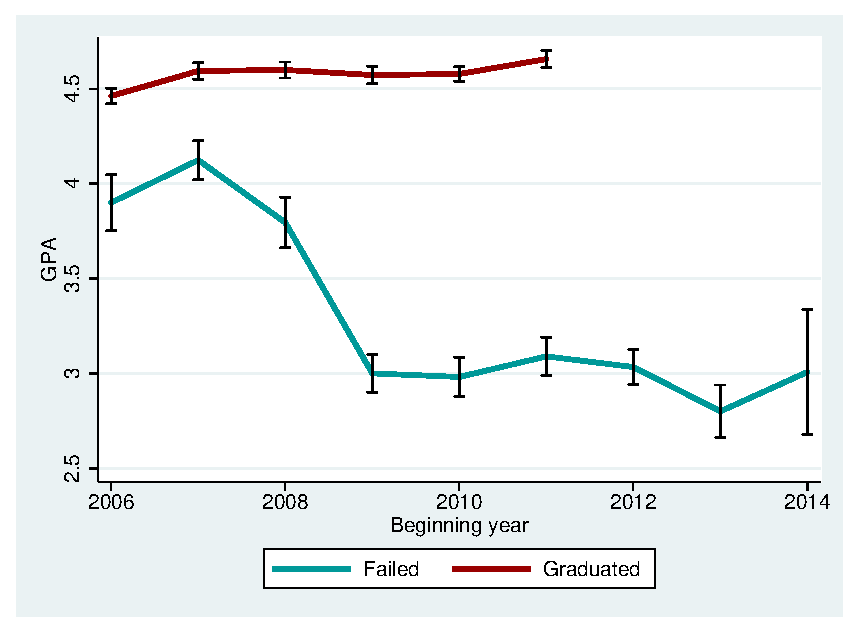
\includegraphics[width=0.6\paperwidth]{img/moyenne.eps}}
\caption{Moyenne par année et par état du cursus (gradué vs. échec/abandon)}
\label{fig:moyenne}
\end{figure}


\begin{figure}[H]
\makebox[\textwidth][c]{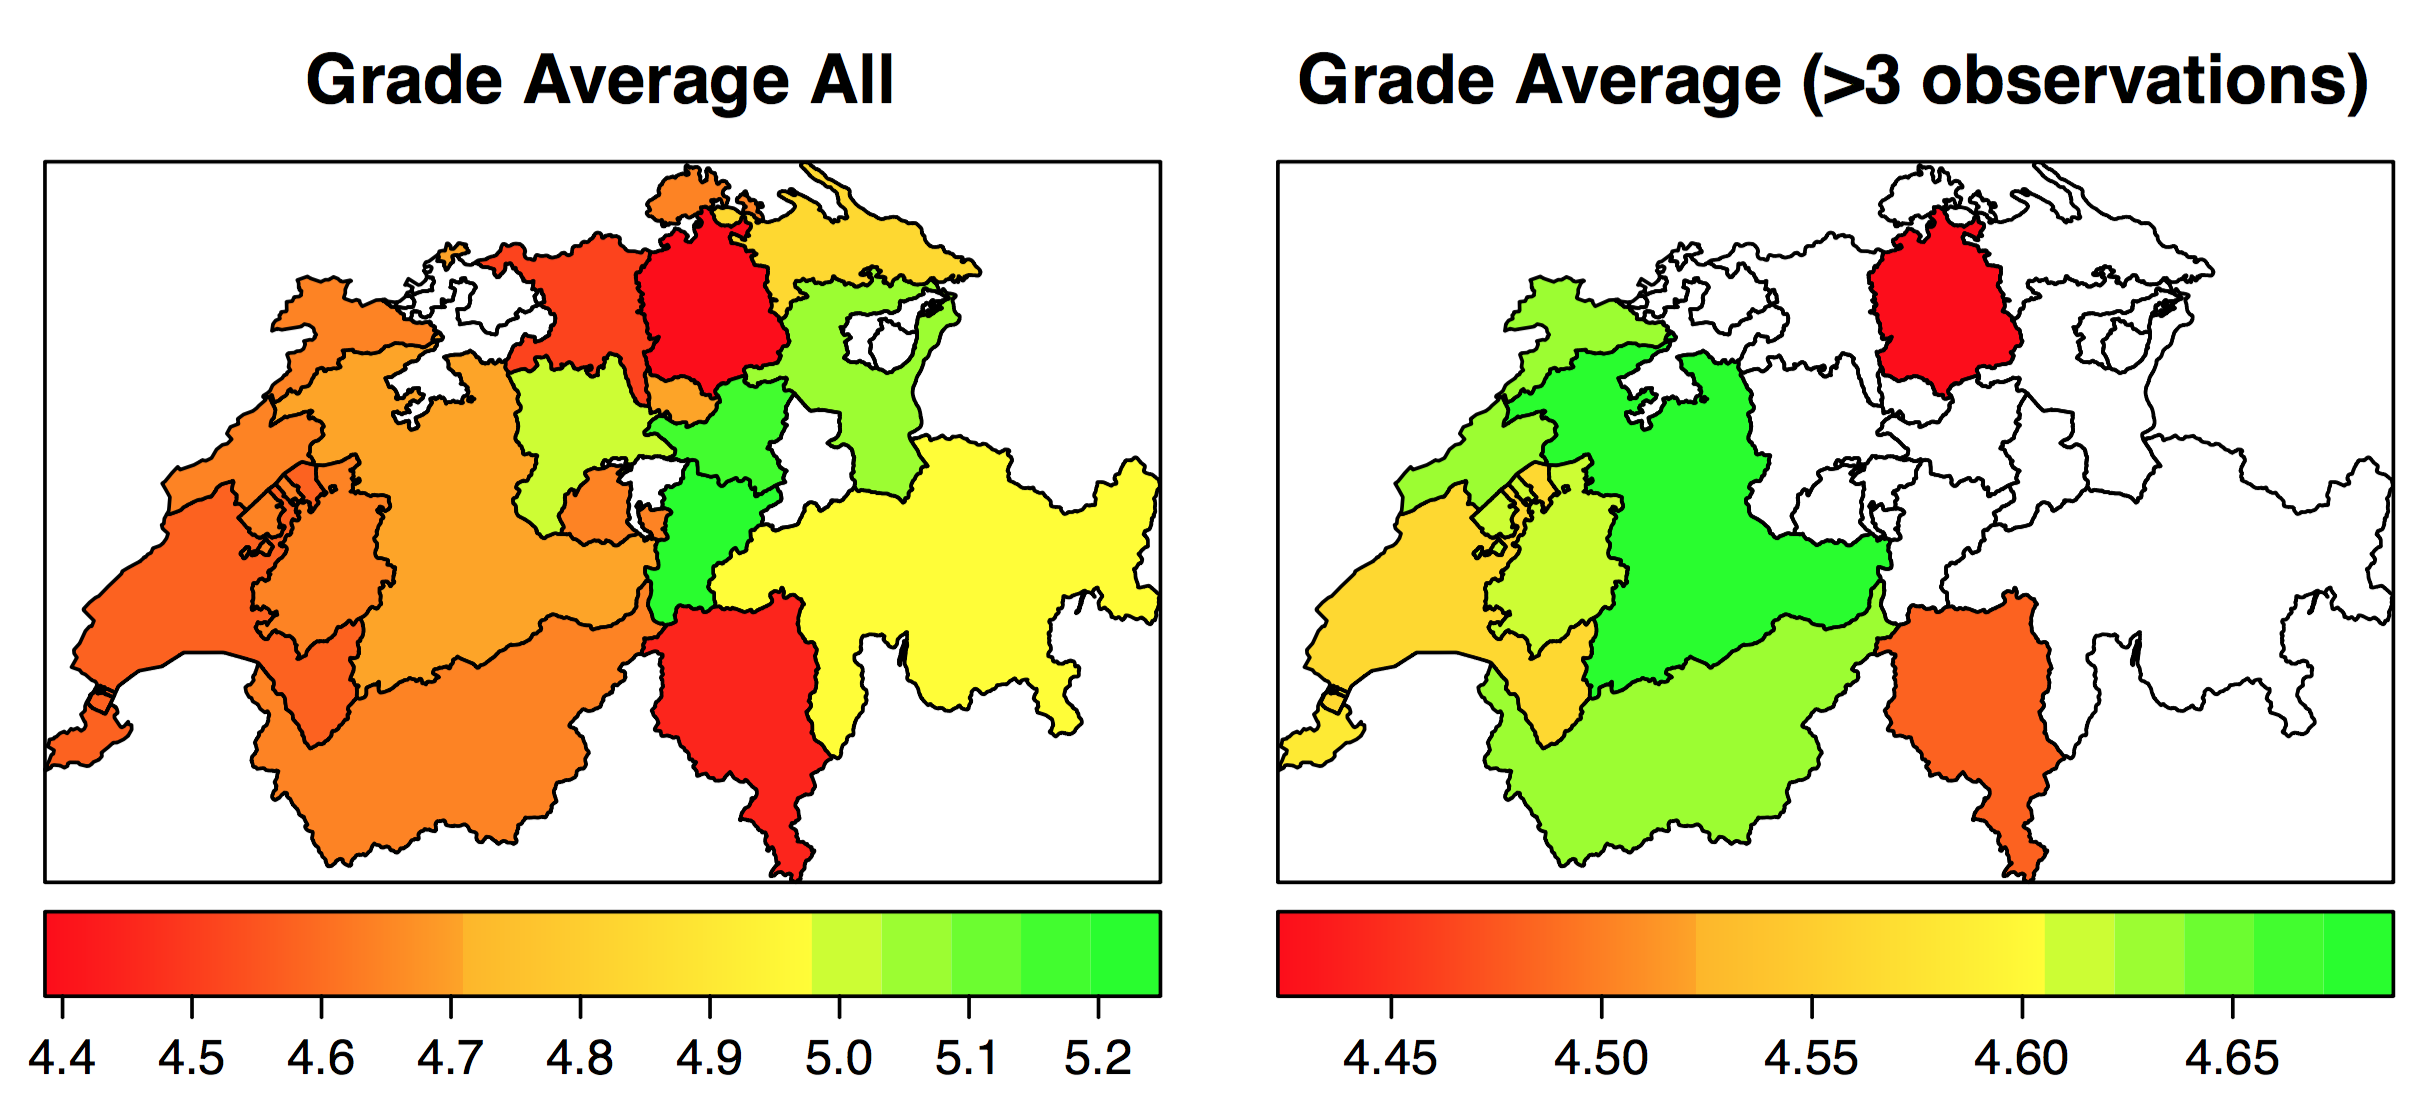
\includegraphics[width=0.9\paperwidth]{img/canton.png}}
\caption{Moyenne au Bachelor par canton de maturité (uniquement cursus réussis)}
\label{fig:canton}
\end{figure}

\begin{figure}[H]
\makebox[\textwidth][c]{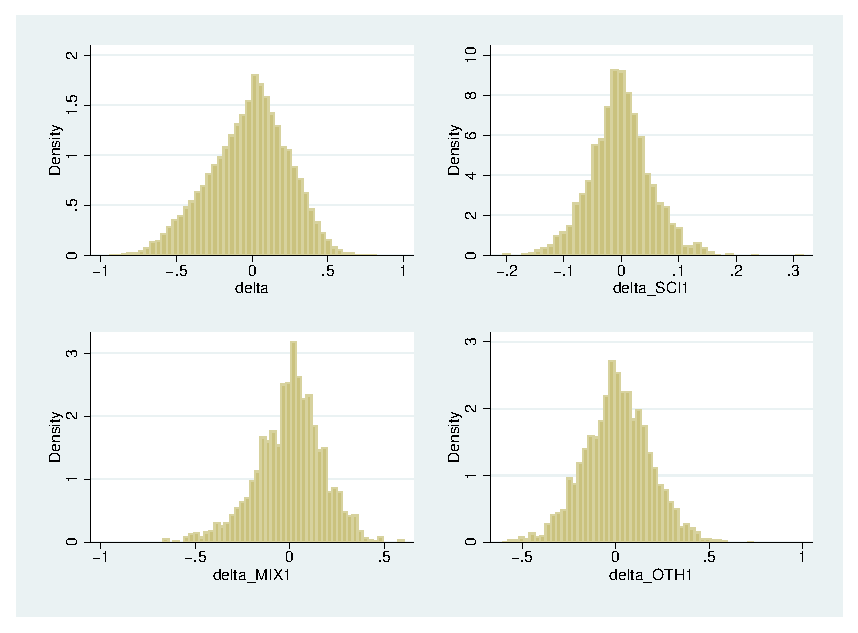
\includegraphics[width=0.75\paperwidth]{img/deltas.eps}}
\caption{Distribution des deltas}
\label{fig:deltas}
\end{figure}

\begin{figure}[H]
\makebox[\textwidth][c]{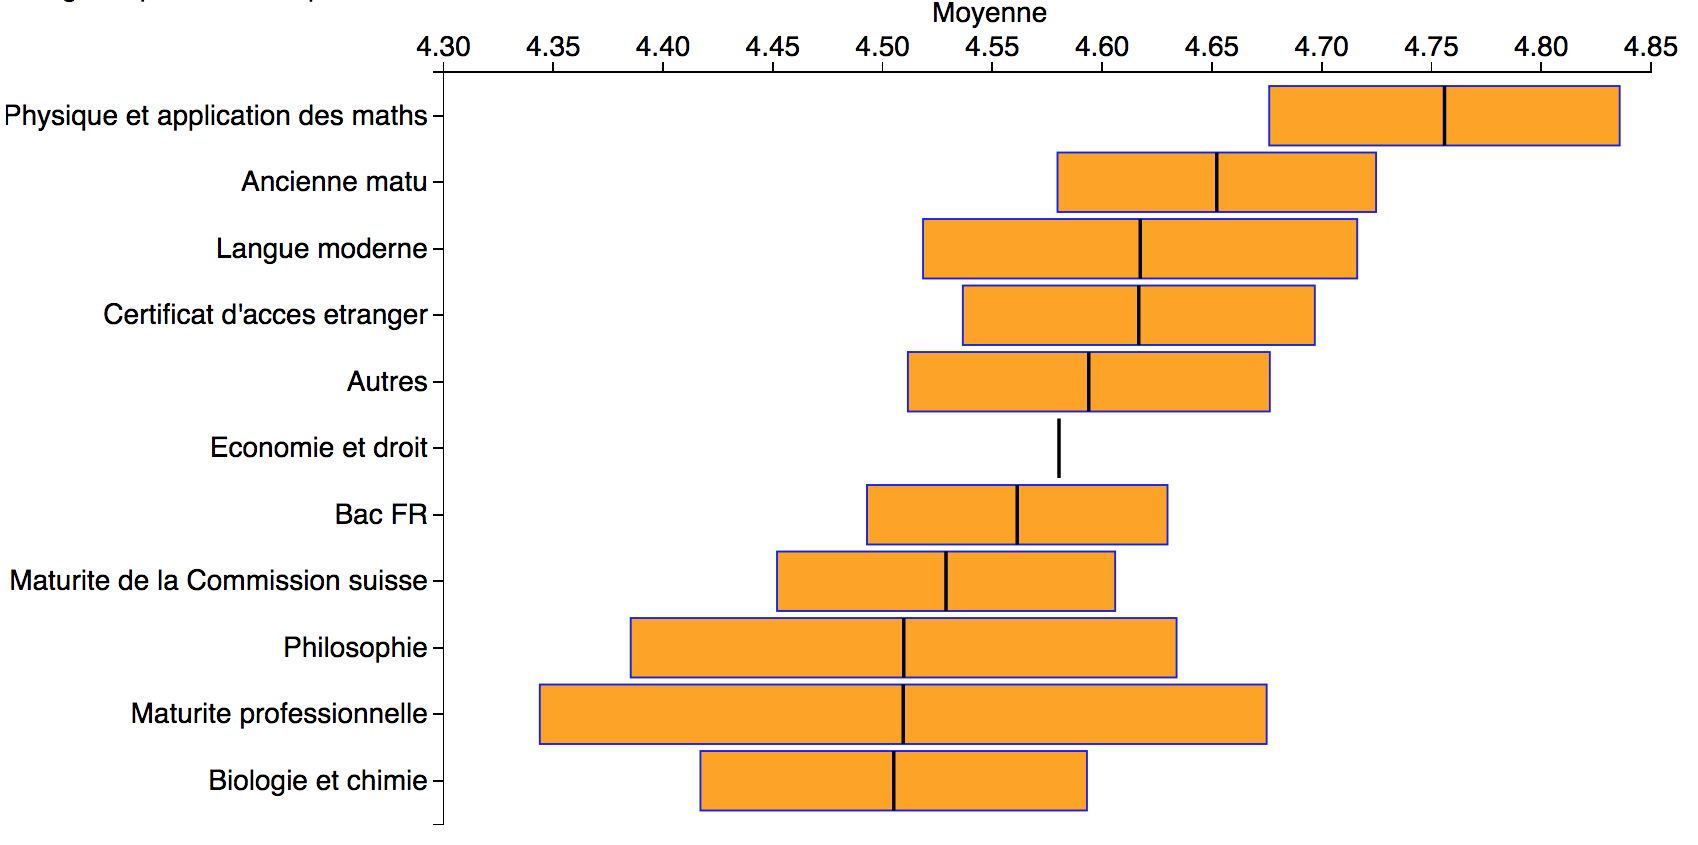
\includegraphics[width=0.8\paperwidth]{img/matu.png}}
\caption{Moyenne au Bachelor par type de maturité (cursus réussis uniquement)}
\label{fig:matu}
\end{figure}

\begin{figure}[H]
\makebox[\textwidth][c]{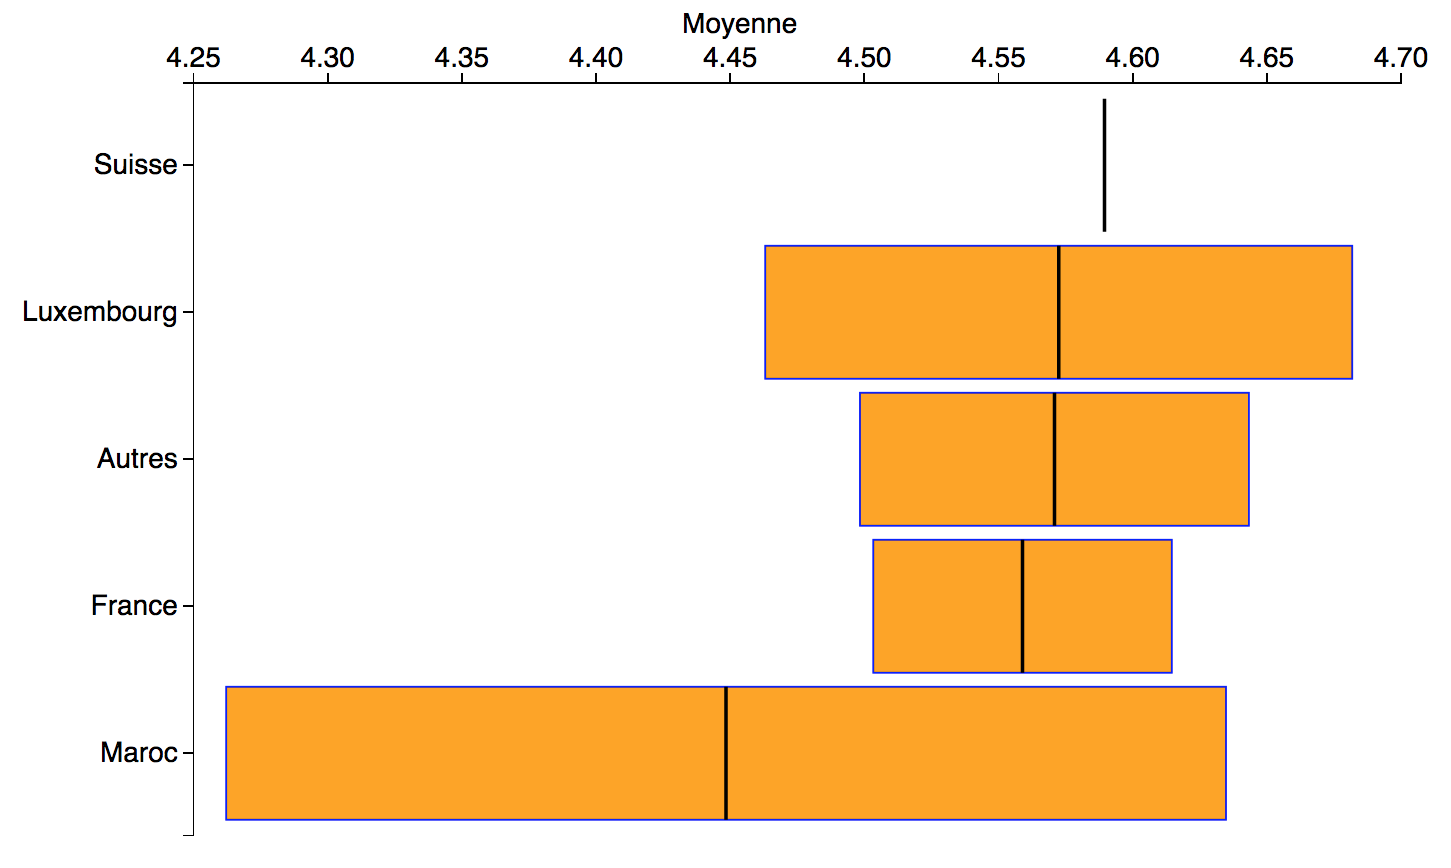
\includegraphics[width=0.95\paperwidth]{img/pays.png}}
\caption{Moyenne au Bachelor par pays d'obtention du diplôme d'accès (cursus réussis uniquement)}
\label{fig:pays}
\end{figure}


\subsection{tableaux}
\subsubsection{Données}

\begin{table}[H]
\begin{center}
\begin{tabular}{l  c  c  c  c  c  c }\hline\hline
\multicolumn{1}{c}{Variables} &delta\_OTH1&delta\_OTH23&delta\_SCI1&delta\_SCI23&delta\_MIX1&delta\_MIX23\\ \hline
delta\_OTH1&1.000\\
delta\_OTH23&0.300&1.000\\
delta\_SCI1&-0.669&-0.184&1.000\\
delta\_SCI23&-0.273&-0.812&0.218&1.000\\
delta\_MIX1&-0.069&-0.042&-0.685&-0.030&1.000\\
delta\_MIX23&-0.095&-0.313&-0.072&-0.080&0.184&1.000\\
\hline \hline 
 \end{tabular}
 \end{center}

\caption{Corrélation entre les delta des différentes catégories}
\label{tab:corr}
\end{table}

\begin{table}[H]
\begin{center}
\begin{tabular}{lcccccc} \hline
 & (1) & (2) & (3) & (4) & (5) & (6) \\
VARIABLES & delta\_SCI23 & delta\_SCI23 & delta\_SCI23 & delta\_SCI23 & delta\_SCI23 & delta\_SCI23 \\ \hline
\vspace{4pt} & \begin{footnotesize}\end{footnotesize} & \begin{footnotesize}\end{footnotesize} & \begin{footnotesize}\end{footnotesize} & \begin{footnotesize}\end{footnotesize} & \begin{footnotesize}\end{footnotesize} & \begin{footnotesize}\end{footnotesize} \\
delta\_SCI1 & 0.339*** &  & 0.066** & 0.207*** &  &  \\
\vspace{4pt} & \begin{footnotesize}(0.032)\end{footnotesize} & \begin{footnotesize}\end{footnotesize} & \begin{footnotesize}(0.032)\end{footnotesize} & \begin{footnotesize}(0.024)\end{footnotesize} & \begin{footnotesize}\end{footnotesize} & \begin{footnotesize}\end{footnotesize} \\
delta\_MIX1 & 0.060*** & -0.016** &  &  & -0.011 &  \\
\vspace{4pt} & \begin{footnotesize}(0.010)\end{footnotesize} & \begin{footnotesize}(0.007)\end{footnotesize} & \begin{footnotesize}\end{footnotesize} & \begin{footnotesize}\end{footnotesize} & \begin{footnotesize}(0.008)\end{footnotesize} & \begin{footnotesize}\end{footnotesize} \\
delta\_OTH1 &  & -0.077*** & -0.062*** &  &  & -0.076*** \\
\vspace{4pt} & \begin{footnotesize}\end{footnotesize} & \begin{footnotesize}(0.007)\end{footnotesize} & \begin{footnotesize}(0.010)\end{footnotesize} & \begin{footnotesize}\end{footnotesize} & \begin{footnotesize}\end{footnotesize} & \begin{footnotesize}(0.007)\end{footnotesize} \\
Constant & -0.015*** & -0.015*** & -0.015*** & -0.016*** & -0.016*** & -0.015*** \\
 & \begin{footnotesize}(0.003)\end{footnotesize} & \begin{footnotesize}(0.003)\end{footnotesize} & \begin{footnotesize}(0.003)\end{footnotesize} & \begin{footnotesize}(0.003)\end{footnotesize} & \begin{footnotesize}(0.003)\end{footnotesize} & \begin{footnotesize}(0.003)\end{footnotesize} \\
\vspace{4pt} & \begin{footnotesize}\end{footnotesize} & \begin{footnotesize}\end{footnotesize} & \begin{footnotesize}\end{footnotesize} & \begin{footnotesize}\end{footnotesize} & \begin{footnotesize}\end{footnotesize} & \begin{footnotesize}\end{footnotesize} \\
Observations & 1,896 & 1,896 & 1,896 & 1,897 & 1,896 & 1,896 \\
 $R^2$ & 0.079 & 0.082 & 0.081 & 0.060 & 0.020 & 0.079 \\ \hline
\multicolumn{7}{c}{\begin{footnotesize} Robust standard errors in parentheses\end{footnotesize}} \\
\multicolumn{7}{c}{\begin{footnotesize} *** p$<$0.01, ** p$<$0.05, * p$<$0.1\end{footnotesize}} \\
\end{tabular}
\end{center}

\caption{Différentes combinaisons de régresseurs expliquant les résultats quantitatifs de 2ème et 3ème année}
\label{tab:sci23}
\end{table}

\begin{table}[H]
\begin{center}
\begin{tabular}{lcccccc} \hline
 & (1) & (2) & (3) & (4) & (5) & (6) \\
VARIABLES & delta\_MIX23 & delta\_MIX23 & delta\_MIX23 & delta\_MIX23 & delta\_MIX23 & delta\_MIX23 \\ \hline
\vspace{4pt} & \begin{footnotesize}\end{footnotesize} & \begin{footnotesize}\end{footnotesize} & \begin{footnotesize}\end{footnotesize} & \begin{footnotesize}\end{footnotesize} & \begin{footnotesize}\end{footnotesize} & \begin{footnotesize}\end{footnotesize} \\
delta\_SCI1 & 0.318*** &  & -0.761*** & -0.245*** &  &  \\
\vspace{4pt} & \begin{footnotesize}(0.112)\end{footnotesize} & \begin{footnotesize}\end{footnotesize} & \begin{footnotesize}(0.112)\end{footnotesize} & \begin{footnotesize}(0.085)\end{footnotesize} & \begin{footnotesize}\end{footnotesize} & \begin{footnotesize}\end{footnotesize} \\
delta\_MIX1 & 0.237*** & 0.168*** &  &  & 0.172*** &  \\
\vspace{4pt} & \begin{footnotesize}(0.033)\end{footnotesize} & \begin{footnotesize}(0.025)\end{footnotesize} & \begin{footnotesize}\end{footnotesize} & \begin{footnotesize}\end{footnotesize} & \begin{footnotesize}(0.025)\end{footnotesize} & \begin{footnotesize}\end{footnotesize} \\
delta\_OTH1 &  & -0.072*** & -0.236*** &  &  & -0.083*** \\
\vspace{4pt} & \begin{footnotesize}\end{footnotesize} & \begin{footnotesize}(0.024)\end{footnotesize} & \begin{footnotesize}(0.033)\end{footnotesize} & \begin{footnotesize}\end{footnotesize} & \begin{footnotesize}\end{footnotesize} & \begin{footnotesize}(0.025)\end{footnotesize} \\
Constant & -0.045*** & -0.044*** & -0.044*** & -0.043*** & -0.044*** & -0.042*** \\
 & \begin{footnotesize}(0.010)\end{footnotesize} & \begin{footnotesize}(0.010)\end{footnotesize} & \begin{footnotesize}(0.010)\end{footnotesize} & \begin{footnotesize}(0.010)\end{footnotesize} & \begin{footnotesize}(0.010)\end{footnotesize} & \begin{footnotesize}(0.010)\end{footnotesize} \\
\vspace{4pt} & \begin{footnotesize}\end{footnotesize} & \begin{footnotesize}\end{footnotesize} & \begin{footnotesize}\end{footnotesize} & \begin{footnotesize}\end{footnotesize} & \begin{footnotesize}\end{footnotesize} & \begin{footnotesize}\end{footnotesize} \\
Observations & 1,485 & 1,485 & 1,485 & 1,486 & 1,485 & 1,485 \\
 $R^2$ & 0.054 & 0.055 & 0.055 & 0.018 & 0.049 & 0.020 \\ \hline
\multicolumn{7}{c}{\begin{footnotesize} Robust standard errors in parentheses\end{footnotesize}} \\
\multicolumn{7}{c}{\begin{footnotesize} *** p$<$0.01, ** p$<$0.05, * p$<$0.1\end{footnotesize}} \\
\end{tabular}
\end{center}

\caption{Différentes combinaisons de régresseurs expliquant les résultats mixtes de 2ème et 3ème année}
\label{tab:mix23}
\end{table}

\begin{table}[H]
\begin{center}
\begin{tabular}{lcccccc} \hline
 & (1) & (2) & (3) & (4) & (5) & (6) \\
VARIABLES & delta\_OTH23 & delta\_OTH23 & delta\_OTH23 & delta\_OTH23 & delta\_OTH23 & delta\_OTH23 \\ \hline
\vspace{4pt} & \begin{footnotesize}\end{footnotesize} & \begin{footnotesize}\end{footnotesize} & \begin{footnotesize}\end{footnotesize} & \begin{footnotesize}\end{footnotesize} & \begin{footnotesize}\end{footnotesize} & \begin{footnotesize}\end{footnotesize} \\
delta\_SCI1 & -0.704*** &  & 0.042 & -0.309*** &  &  \\
\vspace{4pt} & \begin{footnotesize}(0.064)\end{footnotesize} & \begin{footnotesize}\end{footnotesize} & \begin{footnotesize}(0.059)\end{footnotesize} & \begin{footnotesize}(0.045)\end{footnotesize} & \begin{footnotesize}\end{footnotesize} & \begin{footnotesize}\end{footnotesize} \\
delta\_MIX1 & -0.166*** & -0.012 &  &  & -0.021 &  \\
\vspace{4pt} & \begin{footnotesize}(0.019)\end{footnotesize} & \begin{footnotesize}(0.013)\end{footnotesize} & \begin{footnotesize}\end{footnotesize} & \begin{footnotesize}\end{footnotesize} & \begin{footnotesize}(0.013)\end{footnotesize} & \begin{footnotesize}\end{footnotesize} \\
delta\_OTH1 &  & 0.151*** & 0.161*** &  &  & 0.152*** \\
\vspace{4pt} & \begin{footnotesize}\end{footnotesize} & \begin{footnotesize}(0.014)\end{footnotesize} & \begin{footnotesize}(0.019)\end{footnotesize} & \begin{footnotesize}\end{footnotesize} & \begin{footnotesize}\end{footnotesize} & \begin{footnotesize}(0.014)\end{footnotesize} \\
Constant & 0.029*** & 0.028*** & 0.028*** & 0.028*** & 0.028*** & 0.028*** \\
 & \begin{footnotesize}(0.005)\end{footnotesize} & \begin{footnotesize}(0.005)\end{footnotesize} & \begin{footnotesize}(0.005)\end{footnotesize} & \begin{footnotesize}(0.005)\end{footnotesize} & \begin{footnotesize}(0.005)\end{footnotesize} & \begin{footnotesize}(0.005)\end{footnotesize} \\
\vspace{4pt} & \begin{footnotesize}\end{footnotesize} & \begin{footnotesize}\end{footnotesize} & \begin{footnotesize}\end{footnotesize} & \begin{footnotesize}\end{footnotesize} & \begin{footnotesize}\end{footnotesize} & \begin{footnotesize}\end{footnotesize} \\
Observations & 1,504 & 1,504 & 1,504 & 1,505 & 1,504 & 1,504 \\
 $R^2$ & 0.104 & 0.103 & 0.102 & 0.050 & 0.020 & 0.102 \\ \hline
\multicolumn{7}{c}{\begin{footnotesize} Robust standard errors in parentheses\end{footnotesize}} \\
\multicolumn{7}{c}{\begin{footnotesize} *** p$<$0.01, ** p$<$0.05, * p$<$0.1\end{footnotesize}} \\
\end{tabular}
\end{center}

\caption{Différentes combinaisons de régresseurs expliquant les résultats non-quantitatifs de 2ème et 3ème année}
\label{tab:oth23}
\end{table}

\subsubsection{Analyse Descriptive}

\begin{table}[H]
\begin{center}
\begin{tabular}{l|lllllllll|l}
Sex \textbackslash Year & 2006 & 2007 & 2008 & 2009 & 2010 & 2011 & 2012 & 2013 & 2014 & Total \\ \hline
Female                  & 38   & 98   & 100  & 161  & 185  & 160  & 79   & 40   & 7    & 868   \\
Male                    & 69   & 157  & 225  & 307  & 355  & 266  & 141  & 64   & 8    & 1592  \\ \hline
Total                   & 107  & 255  & 325  & 468  & 540  & 426  & 220  & 104  & 15   & 2460 
\end{tabular}
\end{center}
\caption{Nombre d'étudiants par année de début d'études et par sexe}
\label{tab:sex}
\end{table}

\begin{table}[H]
\begin{center}
\begin{tabular}{l|lllllllll|l}
Sex \textbackslash Year & 2006 & 2007 & 2008 & 2009 & 2010 & 2011 & 2012 & 2013 & 2014 & Total \\ \hline
Female                  & 3   & 5   & 25  & 69  & 79  & 75  & 79   & 40   & 7    & 382   \\
Male                    & 0   & 2  & 31  & 111  & 141  & 129  & 141  & 64   & 8    & 627  \\ \hline
Total                   & 3  & 7  & 56  & 180  & 220  & 204  & 220  & 104  & 15   & 1009 
\end{tabular}
\end{center}
\caption{Nombre d'échecs par année de début d'études et par sexe}
\label{tab:echec}
\end{table}

\begin{table}[H]
\begin{center}
\begin{tabular} {@{} l r r r r @{}} \\ \hline
\textbf{debut       stats } & \textbf{  moyenne\_1} & \textbf{  moyenne\_2} & \textbf{  moyenne\_3} & \textbf{   moyenne} \\
\hline
2006         mean  &   4.501402 &   4.279907 &   4.645573 &   4.445414 \\
               sd  &   .2809568 &   .2589845 &    .375799 &   .2272078 \\
2007         mean  &   4.656693 &   4.395773 &   4.731806 &   4.580176 \\
               sd  &   .4055913 &   .3679294 &   .4037419 &   .3494174 \\
2008         mean  &   4.467636 &    4.44772 &   4.729236 &    4.45977 \\
               sd  &   .5248893 &    .401483 &   .3866541 &   .4894625 \\
2009         mean  &   3.942467 &    4.40179 &     4.7692 &   3.967276 \\
               sd  &   .9465355 &   .5682065 &   .4055311 &   .9260684 \\
2010         mean  &   3.890507 &   4.190239 &   4.736133 &   3.927183 \\
               sd  &   .9483145 &   .8016987 &   .4191381 &   .9659944 \\
2011         mean  &   3.900892 &   4.067337 &   4.782489 &   3.905968 \\
               sd  &   .9604512 &    .964434 &    .411499 &   .9663516 \\
2012         mean  &   3.066211 &   2.560022 &          . &    3.03406 \\
               sd  &   .7010399 &   .9965333 &          . &   .6963755 \\
2013         mean  &   2.817063 &   2.565217 &          . &   2.801102 \\
               sd  &   .7278487 &   .9345747 &          . &   .7215713 \\
2014         mean  &   2.974286 &   3.346154 &          . &   3.008039 \\
               sd  &   .6854618 &   .6887372 &          . &   .6485544 \\
Total        mean  &   3.959048 &   4.114521 &   4.740324 &   3.958644 \\
               sd  &   .9401786 &   .8787889 &   .4042057 &   .9303458 \\
\hline
\end{tabular}
\end{center}
\caption{Moyennes générales de l'ensemble des étudiants, par année de début d'études}
\label{tab:moyenne}
\end{table}


\begin{table}[H]
\centering
\resizebox{0.85\textwidth}{!}{\begin{minipage}{\textwidth}%
\begin{center}
\begin{tabular} {@{} l r r r r @{}} \\ \hline
\textbf{debut       stats } & \textbf{  moyenne\_1} & \textbf{  moyenne\_2} & \textbf{  moyenne\_3} & \textbf{   moyenne} \\
\hline
2006         mean  &   4.191667 &   3.683333 &          . &        3.9 \\
               sd  &   .1127314 &   .1626601 &          . &   .1305038 \\
2007         mean  &       4.35 &   3.860714 &          . &    4.12381 \\
               sd  &   .2236068 &   .1398341 &          . &   .1384796 \\
2008         mean  &   3.830003 &     3.6325 &          . &   3.794568 \\
               sd  &   .5310385 &   .5133023 &          . &   .5081951 \\
2009         mean  &   3.006446 &   3.472987 &   3.227273 &   3.000671 \\
               sd  &   .6910325 &   .8823782 &          . &   .6798109 \\
2010         mean  &   2.995184 &   3.172762 &          . &   2.981994 \\
               sd  &   .7931328 &   .9667299 &          . &   .7818877 \\
2011         mean  &   3.118651 &   2.999986 &          . &   3.090132 \\
               sd  &   .7616749 &   .9509751 &          . &   .7387486 \\
2012         mean  &   3.066211 &   2.560022 &          . &    3.03406 \\
               sd  &   .7010399 &   .9965333 &          . &   .6963755 \\
2013         mean  &   2.817063 &   2.565217 &          . &   2.801102 \\
               sd  &   .7278487 &   .9345747 &          . &   .7215713 \\
2014         mean  &   2.974286 &   3.346154 &          . &   3.008039 \\
               sd  &   .6854618 &   .6887372 &          . &   .6485544 \\
Total        mean  &   3.078262 &   2.945794 &   3.227273 &   3.056033 \\
               sd  &   .7601009 &    .996804 &          . &   .7433736 \\
\hline
\end{tabular}
\end{center}

\caption{Moyennes générales des étudiants ayant échoué ou abandonné, \\ par année de début d'études}
\label{tab:moyenneFail}
\end{minipage}}%
\end{table}



\begin{table}[H]
\centering
\resizebox{0.85\textwidth}{!}{\begin{minipage}{\textwidth}%
\begin{center}
\begin{tabular} {@{} l r r r r @{}} \\ \hline
\textbf{debut       stats } & \textbf{  moyenne\_1} & \textbf{  moyenne\_2} & \textbf{  moyenne\_3} & \textbf{   moyenne} \\
\hline
2006         mean  &   4.510337 &   4.297115 &   4.645573 &   4.461147 \\
               sd  &   .2794892 &   .2405156 &    .375799 &   .2094803 \\
2007         mean  &   4.665385 &   4.410876 &   4.731806 &   4.593057 \\
               sd  &   .4064646 &   .3610971 &   .4037419 &   .3449896 \\
2008         mean  &   4.601372 &   4.478026 &   4.729236 &   4.598251 \\
               sd  &    .414312 &   .3641911 &   .3866541 &   .3534436 \\
2009         mean  &   4.527479 &   4.527566 &   4.776948 &   4.571404 \\
               sd  &   .5168007 &   .3613039 &   .3914307 &   .3937089 \\
2010         mean  &   4.506042 &   4.511381 &   4.736133 &   4.577001 \\
               sd  &   .3933755 &   .3493058 &   .4191381 &   .3424582 \\
2011         mean  &   4.619707 &   4.581781 &   4.782489 &   4.655655 \\
               sd  &   .3964997 &   .3595548 &    .411499 &   .3399634 \\
Total        mean  &     4.5728 &   4.486645 &   4.741692 &   4.586304 \\
               sd  &    .424179 &   .3586725 &   .4018165 &   .3500494 \\
\hline
\end{tabular}

\end{center}
\caption{Moyennes générales des étudiants ayant réussi leur cursus, \\ par année de début d'études}
\label{tab:moyenneFini}
\end{minipage}}%
\end{table}

\begin{table}[H]
\begin{center}
\begin{tabular} {@{} l r r r r @{}} \\ \hline
\textbf{   debut } & \textbf{     delta} & \textbf{  delta\_SCI1} & \textbf{  delta\_MIX1} & \textbf{  delta\_OTH1} \\
\hline
2006         mean  &  -.0010201 &   .0024821 &  -.0066845 &  -.0056984 \\
               sd  &   .2549929 &   .0595867 &   .2248986 &   .2106151 \\
2007         mean  &  -.0002217 &   .0033251 &  -.0123725 &  -.0027931 \\
               sd  &   .2473213 &   .0613527 &   .2276017 &   .2038183 \\
2008         mean  &   .0030124 &  -.0043152 &  -.0088202 &   .0274503 \\
               sd  &   .2359713 &   .0615961 &    .212184 &   .1919601 \\
2009         mean  &   .0087136 &  -.0024599 &  -.0028229 &   .0203145 \\
               sd  &   .2219427 &   .0399081 &     .13132 &   .1530087 \\
2010         mean  &   .0014787 &  -.0021758 &   .0145661 &   .0007911 \\
               sd  &   .2264081 &   .0466623 &    .139706 &   .1600304 \\
2011         mean  &  -.0002945 &  -.0014327 &   .0112612 &   -.004182 \\
               sd  &   .2175955 &   .0471209 &   .1463528 &   .1492725 \\
2012         mean  &   .0035528 &  -.0053011 &  -.0029394 &   .0291159 \\
               sd  &   .2043771 &   .0543845 &   .1486076 &   .1844625 \\
2013         mean  &   .0053406 &  -.0074005 &  -.0127259 &   .0471383 \\
               sd  &   .2135919 &   .0563327 &   .1876084 &    .191214 \\
2014         mean  &  -.0032677 &   .0040687 &  -.0318605 &  -.0064318 \\
               sd  &   .1876941 &   .0792771 &   .2254533 &   .2605538 \\
Total        mean  &    .002515 &  -.0016027 &   .0011797 &    .008531 \\
               sd  &   .2292595 &   .0516892 &   .1730637 &   .1740549 \\
\hline

\end{tabular}
\end{center}
\caption{Distribution des différents delta par année de début d'études}
\label{tab:deltas}
\end{table}

\subsubsection{Résultats}

\begin{table}[H]
  \centering
  %\setcapwidth{0.6\textwidth}
  \checkoddpage
  \edef\side{\ifoddpage l\else r\fi}%
\resizebox{0.85\textwidth}{!}{
    \begin{minipage}[t]{.45\textwidth}
      \centering
      \begin{center}
\begin{tabular}{lcc} \hline
 & (1) & (2) \\
& quant\_2 & moyenne\_2 \\ \hline
\vspace{4pt} & \begin{footnotesize}\end{footnotesize} & \begin{footnotesize}\end{footnotesize} \\
delta\_SCI1 & 0.485*** & 1.272*** \\
\vspace{4pt} & \begin{footnotesize}(0.116)\end{footnotesize} & \begin{footnotesize}(0.384)\end{footnotesize} \\
delta\_MIX1 & 0.180*** & 0.501*** \\
\vspace{4pt} & \begin{footnotesize}(0.032)\end{footnotesize} & \begin{footnotesize}(0.105)\end{footnotesize} \\
Sexe = 2, M & -0.006 & -0.004 \\
\vspace{4pt} & \begin{footnotesize}(0.010)\end{footnotesize} & \begin{footnotesize}(0.035)\end{footnotesize} \\
Constant & 0.548*** & 4.191*** \\
 & \begin{footnotesize}(0.013)\end{footnotesize} & \begin{footnotesize}(0.048)\end{footnotesize} \\
\vspace{4pt} & \begin{footnotesize}\end{footnotesize} & \begin{footnotesize}\end{footnotesize} \\
Control: Year & Yes & Yes \\ \hline
Observations & 1,909 & 1,909 \\
 $R^2$ & 0.031 & 0.365 \\ \hline
\multicolumn{3}{c}{\begin{footnotesize} Robust standard errors in parentheses\end{footnotesize}} \\
\multicolumn{3}{c}{\begin{footnotesize} *** p$<$0.01, ** p$<$0.05, * p$<$0.1\end{footnotesize}} \\
\end{tabular}
\end{center}

	  \caption{Effets de la surperformance 
      catégorielle \\ sur la moyenne relative et 
      absolue de deuxième \\ année}
      \label{tab:result2}

    \end{minipage}%
    \hfill
    \begin{minipage}[t]{0.45\textwidth}
      \centering
      \begin{center}
\begin{tabular}{lcc} \hline
 & (1) & (2) \\
& quant\_3 & moyenne\_3 \\ \hline
\vspace{4pt} & \begin{footnotesize}\end{footnotesize} & \begin{footnotesize}\end{footnotesize} \\
delta\_SCI1 & -0.258** & -0.264 \\
\vspace{4pt} & \begin{footnotesize}(0.123)\end{footnotesize} & \begin{footnotesize}(0.317)\end{footnotesize} \\
delta\_MIX1 & -0.051 & -0.059 \\
\vspace{4pt} & \begin{footnotesize}(0.035)\end{footnotesize} & \begin{footnotesize}(0.087)\end{footnotesize} \\
Sexe = 2, M & -0.036*** & -0.071*** \\
\vspace{4pt} & \begin{footnotesize}(0.010)\end{footnotesize} & \begin{footnotesize}(0.025)\end{footnotesize} \\
Constant & 0.659*** & 4.783*** \\
 & \begin{footnotesize}(0.012)\end{footnotesize} & \begin{footnotesize}(0.031)\end{footnotesize} \\
\vspace{4pt} & \begin{footnotesize}\end{footnotesize} & \begin{footnotesize}\end{footnotesize} \\
Control: Year & Yes & Yes \\ \hline
Observations & 1,103 & 1,103 \\
 $R^2$ & 0.026 & 0.015 \\ \hline
\multicolumn{3}{c}{\begin{footnotesize} Robust standard errors in parentheses\end{footnotesize}} \\
\multicolumn{3}{c}{\begin{footnotesize} *** p$<$0.01, ** p$<$0.05, * p$<$0.1\end{footnotesize}} \\
\end{tabular}
\end{center}

	  \caption{Effets de la surperformance
      catégorielle \\ sur la moyenne relative et 
      absolue de troisième \\ année}
      \label{tab:result3}
    \end{minipage}%
  }%

\end{table}


\begin{table}[H]
\centering
\resizebox{0.85\textwidth}{!}{\begin{minipage}{\textwidth}%
\begin{center}
\begin{tabular}{lcccccc} \hline
 & (1) & (2) & (3) & (4) & (5) & (6) \\
VARIABLES & quant\_2 & quant\_2 & quant\_2 & quant\_2 & quant\_2 & quant\_2 \\ \hline
\vspace{4pt} & \begin{footnotesize}\end{footnotesize} & \begin{footnotesize}\end{footnotesize} & \begin{footnotesize}\end{footnotesize} & \begin{footnotesize}\end{footnotesize} & \begin{footnotesize}\end{footnotesize} & \begin{footnotesize}\end{footnotesize} \\
delta\_SCI1 & 0.485*** &  & -0.312*** & 0.085 &  &  \\
\vspace{4pt} & \begin{footnotesize}(0.116)\end{footnotesize} & \begin{footnotesize}\end{footnotesize} & \begin{footnotesize}(0.106)\end{footnotesize} & \begin{footnotesize}(0.083)\end{footnotesize} & \begin{footnotesize}\end{footnotesize} & \begin{footnotesize}\end{footnotesize} \\
delta\_MIX1 & 0.180*** & 0.073*** &  &  & 0.079*** &  \\
\vspace{4pt} & \begin{footnotesize}(0.032)\end{footnotesize} & \begin{footnotesize}(0.023)\end{footnotesize} & \begin{footnotesize}\end{footnotesize} & \begin{footnotesize}\end{footnotesize} & \begin{footnotesize}(0.023)\end{footnotesize} & \begin{footnotesize}\end{footnotesize} \\
delta\_OTH1 &  & -0.108*** & -0.176*** &  &  & -0.111*** \\
\vspace{4pt} & \begin{footnotesize}\end{footnotesize} & \begin{footnotesize}(0.025)\end{footnotesize} & \begin{footnotesize}(0.032)\end{footnotesize} & \begin{footnotesize}\end{footnotesize} & \begin{footnotesize}\end{footnotesize} & \begin{footnotesize}(0.025)\end{footnotesize} \\
Constant & 0.548*** & 0.548*** & 0.549*** & 0.547*** & 0.546*** & 0.549*** \\
 & \begin{footnotesize}(0.013)\end{footnotesize} & \begin{footnotesize}(0.013)\end{footnotesize} & \begin{footnotesize}(0.013)\end{footnotesize} & \begin{footnotesize}(0.013)\end{footnotesize} & \begin{footnotesize}(0.013)\end{footnotesize} & \begin{footnotesize}(0.013)\end{footnotesize} \\
\vspace{4pt} & \begin{footnotesize}\end{footnotesize} & \begin{footnotesize}\end{footnotesize} & \begin{footnotesize}\end{footnotesize} & \begin{footnotesize}\end{footnotesize} & \begin{footnotesize}\end{footnotesize} & \begin{footnotesize}\end{footnotesize} \\
Observations & 1,909 & 1,909 & 1,909 & 1,910 & 1,909 & 1,909 \\
 $R^2$ & 0.031 & 0.031 & 0.030 & 0.019 & 0.023 & 0.027 \\ \hline
\multicolumn{7}{c}{\begin{footnotesize} Robust standard errors in parentheses\end{footnotesize}} \\
\multicolumn{7}{c}{\begin{footnotesize} *** p$<$0.01, ** p$<$0.05, * p$<$0.1\end{footnotesize}} \\
\end{tabular}
\end{center}

\caption{Toutes les combinaisons de régresseurs pour (1) du tableau \ref{tab:result2}}
\label{tab:quant2}
\end{minipage}}%
\end{table}


\begin{table}[H]
\begin{center}
\begin{tabular}{lccc} \hline
 & (1) & (2) & (3) \\
VARIABLES & fini & fini & y1 \\ \hline
\vspace{4pt} & \begin{footnotesize}\end{footnotesize} & \begin{footnotesize}\end{footnotesize} & \begin{footnotesize}\end{footnotesize} \\
delta\_SCI1 & 10.372*** &  &  \\
\vspace{4pt} & \begin{footnotesize}(1.456)\end{footnotesize} & \begin{footnotesize}\end{footnotesize} & \begin{footnotesize}\end{footnotesize} \\
delta\_MIX1 & 3.522*** &  &  \\
\vspace{4pt} & \begin{footnotesize}(0.461)\end{footnotesize} & \begin{footnotesize}\end{footnotesize} & \begin{footnotesize}\end{footnotesize} \\
Debut = 2006 & 3.604*** & 3.530*** & 0.455*** \\
\vspace{4pt} & \begin{footnotesize}(0.601)\end{footnotesize} & \begin{footnotesize}(0.596)\end{footnotesize} & \begin{footnotesize}(0.030)\end{footnotesize} \\
Debut = 2007 & 3.614*** & 3.536*** & 0.455*** \\
\vspace{4pt} & \begin{footnotesize}(0.403)\end{footnotesize} & \begin{footnotesize}(0.403)\end{footnotesize} & \begin{footnotesize}(0.028)\end{footnotesize} \\
Debut = 2008 & 1.640*** & 1.593*** & 0.322*** \\
\vspace{4pt} & \begin{footnotesize}(0.185)\end{footnotesize} & \begin{footnotesize}(0.182)\end{footnotesize} & \begin{footnotesize}(0.033)\end{footnotesize} \\
Debut = 2009 & 0.471*** & 0.454*** & 0.110*** \\
\vspace{4pt} & \begin{footnotesize}(0.141)\end{footnotesize} & \begin{footnotesize}(0.140)\end{footnotesize} & \begin{footnotesize}(0.034)\end{footnotesize} \\
Debut = 2010 & 0.357*** & 0.361*** & 0.089*** \\
\vspace{4pt} & \begin{footnotesize}(0.137)\end{footnotesize} & \begin{footnotesize}(0.136)\end{footnotesize} & \begin{footnotesize}(0.033)\end{footnotesize} \\
Debut = 2012, omitted & - & - & - \\
\vspace{4pt} & \begin{footnotesize}\end{footnotesize} & \begin{footnotesize}\end{footnotesize} & \begin{footnotesize}\end{footnotesize} \\
Debut = 2013, omitted & - & - & - \\
\vspace{4pt} & \begin{footnotesize}\end{footnotesize} & \begin{footnotesize}\end{footnotesize} & \begin{footnotesize}\end{footnotesize} \\
Debut = 2014, omitted & - & - & - \\
\vspace{4pt} & \begin{footnotesize}\end{footnotesize} & \begin{footnotesize}\end{footnotesize} & \begin{footnotesize}\end{footnotesize} \\
delta\_OTH1 &  & -2.378*** & -0.441*** \\
\vspace{4pt} & \begin{footnotesize}\end{footnotesize} & \begin{footnotesize}(0.300)\end{footnotesize} & \begin{footnotesize}(0.055)\end{footnotesize} \\
Constant & 0.102 & 0.120 &  \\
 & \begin{footnotesize}(0.104)\end{footnotesize} & \begin{footnotesize}(0.103)\end{footnotesize} & \begin{footnotesize}\end{footnotesize} \\
\vspace{4pt} & \begin{footnotesize}\end{footnotesize} & \begin{footnotesize}\end{footnotesize} & \begin{footnotesize}\end{footnotesize} \\
 Observations & 2,103 & 2,102 & 2,102 \\ \hline
\multicolumn{4}{c}{\begin{footnotesize} Robust standard errors in parentheses\end{footnotesize}} \\
\multicolumn{4}{c}{\begin{footnotesize} *** p$<$0.01, ** p$<$0.05, * p$<$0.1\end{footnotesize}} \\
\end{tabular}
\end{center}

\caption{Probabilité de réussir en fonction des deltas. Référence: début en 2011}
\label{tab:logit}
\end{table}

\begin{table}[H]
  %\setcapwidth{0.6\textwidth}
  \checkoddpage
  \edef\side{\ifoddpage l\else r\fi}%
  \makebox[\textwidth][\side]{%
    \begin{minipage}[t]{.5\textwidth}
      \centering
      \begin{center}
\begin{tabular}{lc} \hline
 & (1) \\
 & quant 2 \\ \hline
\vspace{4pt} & \begin{footnotesize}\end{footnotesize} \\
Management & -0.061*** \\
\vspace{4pt} & \begin{footnotesize}(0.022)\end{footnotesize} \\
Maths & 0.104*** \\
\vspace{4pt} & \begin{footnotesize}(0.039)\end{footnotesize} \\
Compta & 0.127*** \\
\vspace{4pt} & \begin{footnotesize}(0.031)\end{footnotesize} \\
Constant & 0.604*** \\
 & \begin{footnotesize}(0.009)\end{footnotesize} \\
\vspace{4pt} & \begin{footnotesize}\end{footnotesize} \\
Observations & 951 \\
 $R^2$ & 0.042 \\ \hline
\multicolumn{2}{c}{\begin{footnotesize} Robust standard errors in parentheses\end{footnotesize}} \\
\multicolumn{2}{c}{\begin{footnotesize} *** p$<$0.01, ** p$<$0.05, * p$<$0.1\end{footnotesize}} \\
\end{tabular}
\end{center}
	  \caption{Effet de la surperformance par cours de première année sur la moyenne normalisée de deuxième (Plans d'études à examens annuels, avant 2011)}
      \label{tab:oldClasses}

    \end{minipage}%
    \hfill
    \begin{minipage}[t]{0.5\textwidth}
      \centering
      \begin{center}
\begin{tabular}{lc} \hline
 & (1) \\
 & quant 2 \\ \hline
\vspace{4pt} & \begin{footnotesize}\end{footnotesize} \\
Management & -0.037 \\
\vspace{4pt} & \begin{footnotesize}(0.047)\end{footnotesize} \\
compta I & -0.176*** \\
\vspace{4pt} & \begin{footnotesize}(0.059)\end{footnotesize} \\
compta II & 0.122** \\
\vspace{4pt} & \begin{footnotesize}(0.057)\end{footnotesize} \\
Prog & -0.143** \\
\vspace{4pt} & \begin{footnotesize}(0.063)\end{footnotesize} \\
Droit 1er & -0.209*** \\
\vspace{4pt} & \begin{footnotesize}(0.046)\end{footnotesize} \\
Droit 2e & 0.033 \\
\vspace{4pt} & \begin{footnotesize}(0.051)\end{footnotesize} \\
Modeles Info & -0.252*** \\
\vspace{4pt} & \begin{footnotesize}(0.062)\end{footnotesize} \\
Stats I & -0.130** \\
\vspace{4pt} & \begin{footnotesize}(0.057)\end{footnotesize} \\
Stats II & 0.089 \\
\vspace{4pt} & \begin{footnotesize}(0.060)\end{footnotesize} \\
Constant & 0.610*** \\
 & \begin{footnotesize}(0.017)\end{footnotesize} \\
\vspace{4pt} & \begin{footnotesize}\end{footnotesize} \\
Observations & 551 \\
 $R^2$ & 0.175 \\ \hline
\multicolumn{2}{c}{\begin{footnotesize} Robust standard errors in parentheses\end{footnotesize}} \\
\multicolumn{2}{c}{\begin{footnotesize} *** p$<$0.01, ** p$<$0.05, * p$<$0.1\end{footnotesize}} \\
\end{tabular}
\end{center}
	  \caption{Effet de la surperformance par cours de première année sur la moyenne normalisée de deuxième (Plans d'études à examens semestriels, dès 2011)}
      \label{tab:newClasses}
    \end{minipage}%
  }%
\end{table}

\begin{table}[H]
\centering
\resizebox{0.85\textwidth}{!}{\begin{minipage}{\textwidth}%
\begin{center}
\begin{tabular}{lcc} \hline
 & (1) & (2) \\
 & moyenne 2e & moyenne 3e \\ \hline
\vspace{4pt} & \begin{footnotesize}\end{footnotesize} & \begin{footnotesize}\end{footnotesize} \\
Male & -0.030 & -0.088*** \\
\vspace{4pt} & \begin{footnotesize}(0.029)\end{footnotesize} & \begin{footnotesize}(0.024)\end{footnotesize} \\
Echec. & -1.484*** &  \\
\vspace{4pt} & \begin{footnotesize}(0.047)\end{footnotesize} & \begin{footnotesize}\end{footnotesize} \\
Bach. Eco. & 0.273*** & 0.223*** \\
\vspace{4pt} & \begin{footnotesize}(0.025)\end{footnotesize} & \begin{footnotesize}(0.034)\end{footnotesize} \\
Constant & 4.443*** & 4.757*** \\
 & \begin{footnotesize}(0.020)\end{footnotesize} & \begin{footnotesize}(0.019)\end{footnotesize} \\
\vspace{4pt} & \begin{footnotesize}\end{footnotesize} & \begin{footnotesize}\end{footnotesize} \\
Observations & 1,913 & 1,107 \\
 $R^2$ & 0.579 & 0.053 \\ \hline
\multicolumn{3}{c}{\begin{footnotesize} Robust standard errors in parentheses\end{footnotesize}} \\
\multicolumn{3}{c}{\begin{footnotesize} *** p$<$0.01, ** p$<$0.05, * p$<$0.1\end{footnotesize}} \\
\end{tabular}
\end{center}
\caption{Distinction entre les orientations de troisième année (référence: Management)}
\label{tab:bac}
\end{minipage}}%
\end{table}

\begin{table}[H]
\centering
\resizebox{0.85\textwidth}{!}{\begin{minipage}{\textwidth}%
\begin{center}
\begin{tabular}{lcccc} \hline
 & (1) & (2) & (3) & (4) \\
Moyenne & Tous & Tous & Bachelor réussi & Bachelor réussi \\ \hline
\vspace{4pt} & \begin{footnotesize}\end{footnotesize} & \begin{footnotesize}\end{footnotesize} & \begin{footnotesize}\end{footnotesize} & \begin{footnotesize}\end{footnotesize} \\
Male & 0.052 & 0.048 & 0.004 & 0.006 \\
\vspace{4pt} & \begin{footnotesize}(0.039)\end{footnotesize} & \begin{footnotesize}(0.034)\end{footnotesize} & \begin{footnotesize}(0.019)\end{footnotesize} & \begin{footnotesize}(0.019)\end{footnotesize} \\
Autres & -0.479*** & -0.311*** & -0.020 & -0.019 \\
\vspace{4pt} & \begin{footnotesize}(0.084)\end{footnotesize} & \begin{footnotesize}(0.072)\end{footnotesize} & \begin{footnotesize}(0.038)\end{footnotesize} & \begin{footnotesize}(0.037)\end{footnotesize} \\
France & -0.250*** & -0.143*** & -0.029 & -0.031 \\
\vspace{4pt} & \begin{footnotesize}(0.054)\end{footnotesize} & \begin{footnotesize}(0.046)\end{footnotesize} & \begin{footnotesize}(0.029)\end{footnotesize} & \begin{footnotesize}(0.028)\end{footnotesize} \\
Luxembourg & -0.136 & -0.118 & -0.004 & -0.017 \\
\vspace{4pt} & \begin{footnotesize}(0.137)\end{footnotesize} & \begin{footnotesize}(0.133)\end{footnotesize} & \begin{footnotesize}(0.055)\end{footnotesize} & \begin{footnotesize}(0.056)\end{footnotesize} \\
Maroc & -0.944*** & -0.627*** & -0.166* & -0.141 \\
\vspace{4pt} & \begin{footnotesize}(0.125)\end{footnotesize} & \begin{footnotesize}(0.116)\end{footnotesize} & \begin{footnotesize}(0.096)\end{footnotesize} & \begin{footnotesize}(0.095)\end{footnotesize} \\
Constant & 4.021*** & 3.963*** & 4.590*** & 4.581*** \\
 & \begin{footnotesize}(0.033)\end{footnotesize} & \begin{footnotesize}(0.047)\end{footnotesize} & \begin{footnotesize}(0.017)\end{footnotesize} & \begin{footnotesize}(0.024)\end{footnotesize} \\
\vspace{4pt} & \begin{footnotesize}\end{footnotesize} & \begin{footnotesize}\end{footnotesize} & \begin{footnotesize}\end{footnotesize} & \begin{footnotesize}\end{footnotesize} \\
Control: Year & No & Yes & No & Yes \\ \hline
Observations & 2,460 & 2,460 & 1,451 & 1,451 \\
 $R^2$ & 0.046 & 0.277 & 0.003 & 0.018 \\ \hline
\multicolumn{5}{c}{\begin{footnotesize} Robust standard errors in parentheses\end{footnotesize}} \\
\multicolumn{5}{c}{\begin{footnotesize} *** p$<$0.01, ** p$<$0.05, * p$<$0.1\end{footnotesize}} \\
\end{tabular}
\end{center}

\caption{Moyenne (avec et sans échecs) en fonction du pays de maturité. Référence: Suisse, 2010}
\label{tab:matuLieu}
\end{minipage}}%
\end{table}

\begin{table}[H]
\begin{center}
\begin{tabular}{lcccc} \hline
 & (1) & (2) & (3) & (4) \\
Moyenne & Tous & Tous & Bachelor réussi & Bachelor réussi \\ \hline
\vspace{4pt} & \begin{footnotesize}\end{footnotesize} & \begin{footnotesize}\end{footnotesize} & \begin{footnotesize}\end{footnotesize} & \begin{footnotesize}\end{footnotesize} \\
Male & 0.015 & 0.017 & -0.003 & -0.002 \\
\vspace{4pt} & \begin{footnotesize}(0.037)\end{footnotesize} & \begin{footnotesize}(0.034)\end{footnotesize} & \begin{footnotesize}(0.019)\end{footnotesize} & \begin{footnotesize}(0.019)\end{footnotesize} \\
Autres & -0.563*** & -0.420*** & 0.002 & 0.014 \\
\vspace{4pt} & \begin{footnotesize}(0.085)\end{footnotesize} & \begin{footnotesize}(0.077)\end{footnotesize} & \begin{footnotesize}(0.043)\end{footnotesize} & \begin{footnotesize}(0.042)\end{footnotesize} \\
Bac FR & -0.593*** & -0.394*** & -0.017 & -0.019 \\
\vspace{4pt} & \begin{footnotesize}(0.060)\end{footnotesize} & \begin{footnotesize}(0.057)\end{footnotesize} & \begin{footnotesize}(0.035)\end{footnotesize} & \begin{footnotesize}(0.035)\end{footnotesize} \\
Certificat d'accès étranger & 0.254*** & -0.319*** & -0.006 & 0.036 \\
\vspace{4pt} & \begin{footnotesize}(0.059)\end{footnotesize} & \begin{footnotesize}(0.064)\end{footnotesize} & \begin{footnotesize}(0.034)\end{footnotesize} & \begin{footnotesize}(0.041)\end{footnotesize} \\
Diplôme de fin d'études secondaires & -0.257 & -0.196 & 0.002 & -0.012 \\
\vspace{4pt} & \begin{footnotesize}(0.164)\end{footnotesize} & \begin{footnotesize}(0.165)\end{footnotesize} & \begin{footnotesize}(0.066)\end{footnotesize} & \begin{footnotesize}(0.066)\end{footnotesize} \\
Maturité de la Commission suisse & -0.393*** & -0.474*** & -0.067* & -0.051 \\
\vspace{4pt} & \begin{footnotesize}(0.079)\end{footnotesize} & \begin{footnotesize}(0.072)\end{footnotesize} & \begin{footnotesize}(0.038)\end{footnotesize} & \begin{footnotesize}(0.039)\end{footnotesize} \\
Biologie et chimie & -0.270*** & -0.195** & -0.076* & -0.075* \\
\vspace{4pt} & \begin{footnotesize}(0.085)\end{footnotesize} & \begin{footnotesize}(0.079)\end{footnotesize} & \begin{footnotesize}(0.045)\end{footnotesize} & \begin{footnotesize}(0.045)\end{footnotesize} \\
Langue moderne & -0.314*** & -0.220*** & 0.037 & 0.037 \\
\vspace{4pt} & \begin{footnotesize}(0.095)\end{footnotesize} & \begin{footnotesize}(0.084)\end{footnotesize} & \begin{footnotesize}(0.050)\end{footnotesize} & \begin{footnotesize}(0.050)\end{footnotesize} \\
Philosophie & -0.516*** & -0.371*** & -0.068 & -0.071 \\
\vspace{4pt} & \begin{footnotesize}(0.158)\end{footnotesize} & \begin{footnotesize}(0.118)\end{footnotesize} & \begin{footnotesize}(0.065)\end{footnotesize} & \begin{footnotesize}(0.063)\end{footnotesize} \\
Physique et application des maths & 0.377*** & 0.353*** & 0.181*** & 0.176*** \\
\vspace{4pt} & \begin{footnotesize}(0.062)\end{footnotesize} & \begin{footnotesize}(0.059)\end{footnotesize} & \begin{footnotesize}(0.040)\end{footnotesize} & \begin{footnotesize}(0.041)\end{footnotesize} \\
Maturité professionnelle& -0.205 & -0.126 & -0.075 & -0.071 \\
\vspace{4pt} & \begin{footnotesize}(0.154)\end{footnotesize} & \begin{footnotesize}(0.111)\end{footnotesize} & \begin{footnotesize}(0.085)\end{footnotesize} & \begin{footnotesize}(0.084)\end{footnotesize} \\
Vieille maturité & 0.387*** & -0.236*** & 0.008 & 0.072* \\
\vspace{4pt} & \begin{footnotesize}(0.044)\end{footnotesize} & \begin{footnotesize}(0.061)\end{footnotesize} & \begin{footnotesize}(0.026)\end{footnotesize} & \begin{footnotesize}(0.037)\end{footnotesize} \\
Constant & 4.066*** & 4.100*** & 4.580*** & 4.573*** \\
 & \begin{footnotesize}(0.042)\end{footnotesize} & \begin{footnotesize}(0.052)\end{footnotesize} & \begin{footnotesize}(0.022)\end{footnotesize} & \begin{footnotesize}(0.027)\end{footnotesize} \\
\vspace{4pt} & \begin{footnotesize}\end{footnotesize} & \begin{footnotesize}\end{footnotesize} & \begin{footnotesize}\end{footnotesize} & \begin{footnotesize}\end{footnotesize} \\
Control: Year & No & Yes & No & Yes \\ \hline
Observations & 2,460 & 2,460 & 1,451 & 1,451 \\
 $R^2$ & 0.154 & 0.313 & 0.031 & 0.047 \\ \hline
\multicolumn{5}{c}{\begin{footnotesize} Robust standard errors in parentheses\end{footnotesize}} \\
\multicolumn{5}{c}{\begin{footnotesize} *** p$<$0.01, ** p$<$0.05, * p$<$0.1\end{footnotesize}} \\
\end{tabular}
\end{center}

\caption{Moyenne (avec et sans échecs) en fonction du type de maturité. Référence: Éco-droit, 2010}
\label{tab:matuNom}
\end{table}

\begin{table}[H]
% !TEX encoding = UTF-8 Unicode

\begin{center}
\begin{tabular}{lcc} \hline
 & (1) & (2) \\
Logit & P(S) & Marginal \\ \hline
\vspace{4pt} & \begin{footnotesize}\end{footnotesize} & \begin{footnotesize}\end{footnotesize} \\
Male & 0.103 & 0.019 \\
\vspace{4pt} & \begin{footnotesize}(0.111)\end{footnotesize} & \begin{footnotesize}(0.021)\end{footnotesize} \\
Autres & -0.804*** & -0.139*** \\
\vspace{4pt} & \begin{footnotesize}(0.210)\end{footnotesize} & \begin{footnotesize}(0.041)\end{footnotesize} \\
Bac FR & -0.931*** & -0.166*** \\
\vspace{4pt} & \begin{footnotesize}(0.154)\end{footnotesize} & \begin{footnotesize}(0.030)\end{footnotesize} \\
Certificat d'accès étranger & -1.301*** & -0.252*** \\
\vspace{4pt} & \begin{footnotesize}(0.260)\end{footnotesize} & \begin{footnotesize}(0.056)\end{footnotesize} \\
Diplôme de fin d'études secondaires & -0.397 & -0.061 \\
\vspace{4pt} & \begin{footnotesize}(0.388)\end{footnotesize} & \begin{footnotesize}(0.066)\end{footnotesize} \\
Maturité de la Commission suisse & -1.104*** & -0.205*** \\
\vspace{4pt} & \begin{footnotesize}(0.198)\end{footnotesize} & \begin{footnotesize}(0.042)\end{footnotesize} \\
Biologie et chimie & -0.413* & -0.064* \\
\vspace{4pt} & \begin{footnotesize}(0.216)\end{footnotesize} & \begin{footnotesize}(0.036)\end{footnotesize} \\
Langue moderne & -0.604** & -0.099** \\
\vspace{4pt} & \begin{footnotesize}(0.243)\end{footnotesize} & \begin{footnotesize}(0.045)\end{footnotesize} \\
Philosophie & -0.764 & -0.131 \\
\vspace{4pt} & \begin{footnotesize}(0.485)\end{footnotesize} & \begin{footnotesize}(0.099)\end{footnotesize} \\
Physique et application des maths & 0.545** & 0.061*** \\
\vspace{4pt} & \begin{footnotesize}(0.227)\end{footnotesize} & \begin{footnotesize}(0.023)\end{footnotesize} \\
Maturité professionnelle & 0.161 & 0.020 \\
\vspace{4pt} & \begin{footnotesize}(0.479)\end{footnotesize} & \begin{footnotesize}(0.058)\end{footnotesize} \\
Vieille maturité & -0.878*** & -0.155*** \\
\vspace{4pt} & \begin{footnotesize}(0.253)\end{footnotesize} & \begin{footnotesize}(0.049)\end{footnotesize} \\
Constant &  0.780 *** &  \\
 & \begin{footnotesize}(0.147)\end{footnotesize} & \begin{footnotesize}\end{footnotesize} \\
\vspace{4pt} & \begin{footnotesize}\end{footnotesize} & \begin{footnotesize}\end{footnotesize} \\
Control: Year & Yes & Yes \\ \hline
Observations & 2,121 & 2,121 \\ \hline
\multicolumn{3}{c}{\begin{footnotesize} Robust standard errors in parentheses\end{footnotesize}} \\
\multicolumn{3}{c}{\begin{footnotesize} *** p$<$0.01, ** p$<$0.05, * p$<$0.1\end{footnotesize}} \\
\end{tabular}
\end{center}


\caption{Probabilité de réussir en fonction du type de maturité. Référence: Économie et Droit, 2010}
\label{tab:matuNomLogit}
\end{table}


\begin{table}[H]
\begin{center}
\begin{tabular}{lcc} \hline
 & (1) & (2) \\
Logit & P(S) & Marginal \\ \hline
\vspace{4pt} & \begin{footnotesize}\end{footnotesize} & \begin{footnotesize}\end{footnotesize} \\
Male & 0.155 & 0.030 \\
\vspace{4pt} & \begin{footnotesize}(0.107)\end{footnotesize} & \begin{footnotesize}(0.021)\end{footnotesize} \\
Autres & -0.615*** & -0.125*** \\
\vspace{4pt} & \begin{footnotesize}(0.198)\end{footnotesize} & \begin{footnotesize}(0.044)\end{footnotesize} \\
France & -0.483*** & -0.095*** \\
\vspace{4pt} & \begin{footnotesize}(0.142)\end{footnotesize} & \begin{footnotesize}(0.030)\end{footnotesize} \\
Luxembourg & -0.124 & -0.022 \\
\vspace{4pt} & \begin{footnotesize}(0.341)\end{footnotesize} & \begin{footnotesize}(0.064)\end{footnotesize} \\
Maroc & -2.075*** & -0.473*** \\
\vspace{4pt} & \begin{footnotesize}(0.423)\end{footnotesize} & \begin{footnotesize}(0.088)\end{footnotesize} \\
Constant & 3.688*** &  \\
 & \begin{footnotesize}(0.585)\end{footnotesize} & \begin{footnotesize}\end{footnotesize} \\
\vspace{4pt} & \begin{footnotesize}\end{footnotesize} & \begin{footnotesize}\end{footnotesize} \\
Control: Year & Yes & Yes \\ \hline
 Observations & 2,121 & 2,121 \\ \hline
\multicolumn{3}{c}{\begin{footnotesize} Robust standard errors in parentheses\end{footnotesize}} \\
\multicolumn{3}{c}{\begin{footnotesize} *** p$<$0.01, ** p$<$0.05, * p$<$0.1\end{footnotesize}} \\
\end{tabular}
\end{center}

\caption{Probabilité de réussir en fonction du lieu de maturité. Référence: Suisse}
\label{tab:matuLieuLogit}
\end{table}


\begin{table}[H]
\begin{center}
\resizebox*{!}{\dimexpr\textheight-\lineskip\relax}{%
\begin{center}
\begin{tabular}{lcc} \hline
 & (1) & (2) \\
VARIABLES & moyenne & moyenne \\ \hline
\vspace{4pt} & \begin{footnotesize}\end{footnotesize} & \begin{footnotesize}\end{footnotesize} \\
Sexe = 2, M & 0.050 & 0.009 \\
\vspace{4pt} & \begin{footnotesize}(0.034)\end{footnotesize} & \begin{footnotesize}(0.020)\end{footnotesize} \\
matu\_ecole = 0, 0 & -0.047 & 0.003 \\
\vspace{4pt} & \begin{footnotesize}(0.088)\end{footnotesize} & \begin{footnotesize}(0.055)\end{footnotesize} \\
matu\_ecole = 3, Autre ecole & -0.543*** & -0.008 \\
\vspace{4pt} & \begin{footnotesize}(0.165)\end{footnotesize} & \begin{footnotesize}(0.094)\end{footnotesize} \\
matu\_ecole = 6, College Calvin, Geneve & -0.106 & -0.059 \\
\vspace{4pt} & \begin{footnotesize}(0.151)\end{footnotesize} & \begin{footnotesize}(0.107)\end{footnotesize} \\
matu\_ecole = 19, College de l'Abbaye, Saint-Maurice & 0.249* & 0.054 \\
\vspace{4pt} & \begin{footnotesize}(0.134)\end{footnotesize} & \begin{footnotesize}(0.082)\end{footnotesize} \\
matu\_ecole = 38, Ecole des Arches, Lausanne & -0.543*** & -0.245*** \\
\vspace{4pt} & \begin{footnotesize}(0.176)\end{footnotesize} & \begin{footnotesize}(0.088)\end{footnotesize} \\
matu\_ecole = 40, Ecole etrangere & -0.207** & -0.019 \\
\vspace{4pt} & \begin{footnotesize}(0.086)\end{footnotesize} & \begin{footnotesize}(0.054)\end{footnotesize} \\
matu\_ecole = 42, Ecole suisse non codifiee & -0.352*** & -0.180** \\
\vspace{4pt} & \begin{footnotesize}(0.130)\end{footnotesize} & \begin{footnotesize}(0.073)\end{footnotesize} \\
matu\_ecole = 47, Gymnase d'Yverdon, Cheseaux-Noreaz & 0.067 & 0.103 \\
\vspace{4pt} & \begin{footnotesize}(0.127)\end{footnotesize} & \begin{footnotesize}(0.073)\end{footnotesize} \\
matu\_ecole = 48, Gymnase de Beaulieu, Lausanne & 0.189* & -0.020 \\
\vspace{4pt} & \begin{footnotesize}(0.099)\end{footnotesize} & \begin{footnotesize}(0.062)\end{footnotesize} \\
matu\_ecole = 49, Gymnase de Burier, La Tour-de-Peilz & 0.032 & 0.009 \\
\vspace{4pt} & \begin{footnotesize}(0.105)\end{footnotesize} & \begin{footnotesize}(0.063)\end{footnotesize} \\
matu\_ecole = 50, Gymnase de Chamblandes, Pully & 0.110 & 0.009 \\
\vspace{4pt} & \begin{footnotesize}(0.110)\end{footnotesize} & \begin{footnotesize}(0.068)\end{footnotesize} \\
matu\_ecole = 51, Gymnase de Morges, Morges & 0.144 & 0.050 \\
\vspace{4pt} & \begin{footnotesize}(0.105)\end{footnotesize} & \begin{footnotesize}(0.062)\end{footnotesize} \\
matu\_ecole = 52, Gymnase de Nyon, Nyon & 0.134 & 0.012 \\
\vspace{4pt} & \begin{footnotesize}(0.102)\end{footnotesize} & \begin{footnotesize}(0.062)\end{footnotesize} \\
matu\_ecole = 53, Gymnase de la Cite Lausanne & 0.085 & 0.027 \\
\vspace{4pt} & \begin{footnotesize}(0.117)\end{footnotesize} & \begin{footnotesize}(0.073)\end{footnotesize} \\
matu\_ecole = 54, Gymnase du Bugnon, Lausanne & 0.132 & -0.040 \\
\vspace{4pt} & \begin{footnotesize}(0.112)\end{footnotesize} & \begin{footnotesize}(0.066)\end{footnotesize} \\
matu\_ecole = 94, Lycee Denis-de-Rougemont, Neuch�tel & -0.085 & 0.082 \\
\vspace{4pt} & \begin{footnotesize}(0.141)\end{footnotesize} & \begin{footnotesize}(0.079)\end{footnotesize} \\
matu\_ecole = 95, Lycee Jean-Piaget, Neuch�tel & 0.126 & -0.004 \\
\vspace{4pt} & \begin{footnotesize}(0.178)\end{footnotesize} & \begin{footnotesize}(0.088)\end{footnotesize} \\
matu\_ecole = 96, Lycee cantonal et Ecole superieure de commerce, Po & 0.099 & 0.054 \\
\vspace{4pt} & \begin{footnotesize}(0.169)\end{footnotesize} & \begin{footnotesize}(0.112)\end{footnotesize} \\
matu\_ecole = 97, Lycee-College de La Planta, Sion & 0.352*** & 0.122 \\
\vspace{4pt} & \begin{footnotesize}(0.128)\end{footnotesize} & \begin{footnotesize}(0.098)\end{footnotesize} \\
matu\_ecole = 98, Lycee-College des Creusets, Sion & 0.070 & 0.018 \\
\vspace{4pt} & \begin{footnotesize}(0.107)\end{footnotesize} & \begin{footnotesize}(0.068)\end{footnotesize} \\
Constant & 3.937*** & 4.572*** \\
 & \begin{footnotesize}(0.091)\end{footnotesize} & \begin{footnotesize}(0.053)\end{footnotesize} \\
\vspace{4pt} & \begin{footnotesize}\end{footnotesize} & \begin{footnotesize}\end{footnotesize} \\
Observations & 2,460 & 1,451 \\
 $R^2$ & 0.295 & 0.034 \\ \hline
\multicolumn{3}{c}{\begin{footnotesize} Robust standard errors in parentheses\end{footnotesize}} \\
\multicolumn{3}{c}{\begin{footnotesize} *** p$<$0.01, ** p$<$0.05, * p$<$0.1\end{footnotesize}} \\
\end{tabular}
\end{center}

}%
\caption{Moyenne (avec et sans échecs) en fonction du gymnase. Référence: Beaulieu, 2010}
\label{tab:matuEcole}
\end{center}
\end{table}


\subsubsection{Sondage}

\begin{figure}[H]
\makebox[\textwidth][c]{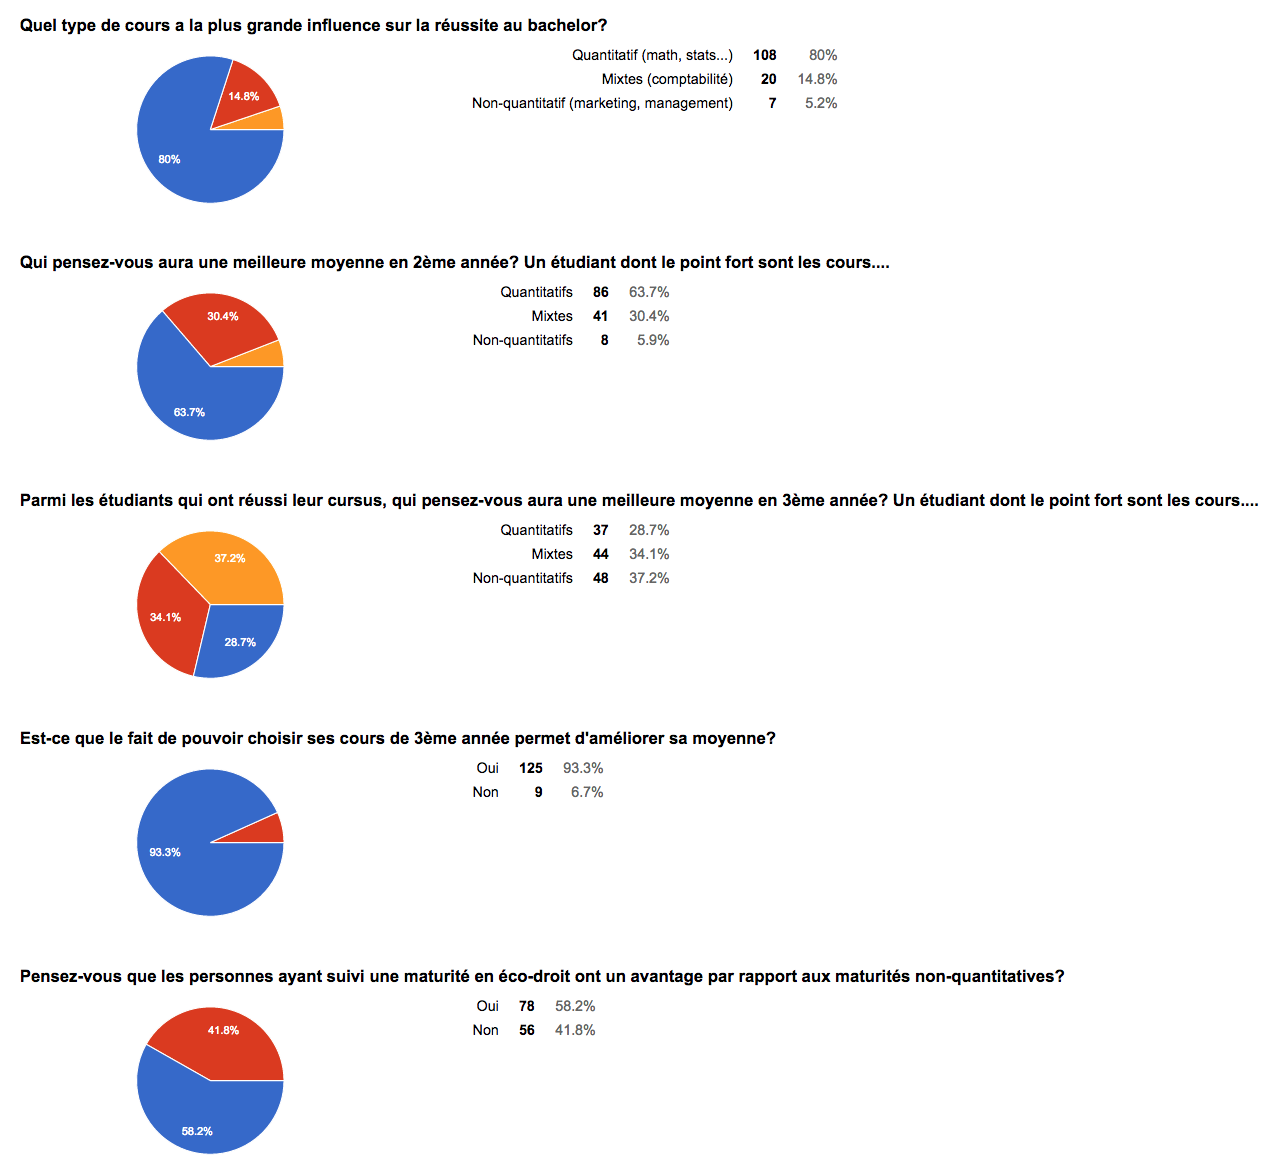
\includegraphics[width=0.9\paperwidth]{img/sondage1.png}}
\caption{Résultats de notre sondage}
\label{fig:sondage1}
\end{figure}

\vfill
\pagebreak

\begin{figure}[H]
\makebox[\textwidth][c]{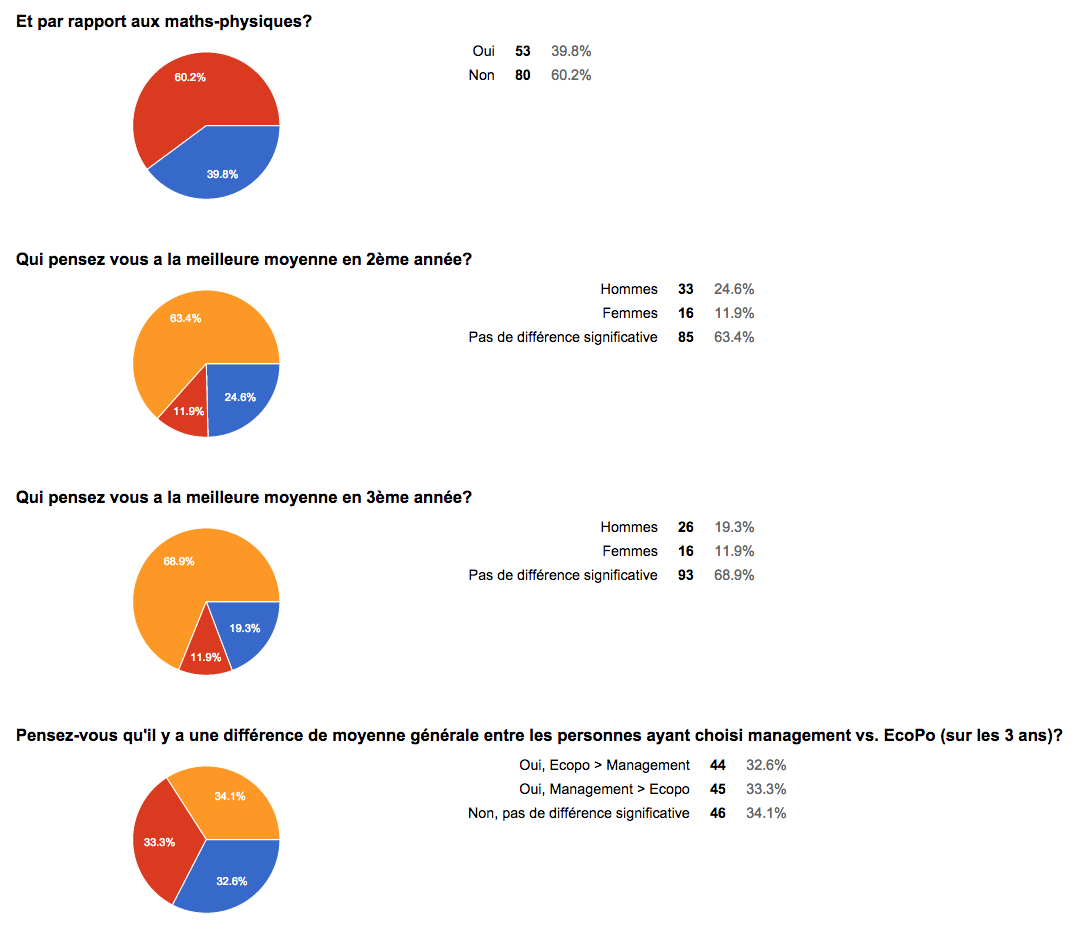
\includegraphics[width=0.9\paperwidth]{img/sondage2.png}}
\caption{Résultats de notre sondage (suite)}
\label{fig:sondage2}
\end{figure}



\end{document}